

The Kirchhoff approximation is used to derive scattering solutions from surfaces or facets that are assumed to be locally smooth, \cite{kong1986electromagnetic}. The idea of locally smooth is usually expressed as a constraint on the minimum local radius of curvature of a rough surface relative to the wavelength, or to say that the correlation length of the surface must be many times larger than the root mean squared height. The core idea of the Kirchhoff approximation is to replace the total electrical and magnetic field solutions at a dielectric interface with Fresnel reflection, rather than to solve the full multiple scattering problem. This formulation can be used to derive the radar cross sections of simple shapes (rectangles, circular disks, etc.), or isolated facets that are used to create larger surface discretizations.

In this chapter, we 1) give the main steps of the Kirchhoff approximation based on \cite{kong1986electromagnetic}, 2) give code for the Fresnel reflection coefficients, 3) give solutions for the surface phase integral over canonical facet shapes, 4) derive expressions for the S-matrix of an arbitrarily shaped surface facet, and 5) derive the equations for specular and backscatter radar cross sections of canonical shapes.


\section{Derivation of the Kirchhoff Approximation}

Let the incident field be a plane wave defined relative to the origin
\eq{\bb{E}_i = \bb{e}_i E_o e^{i\bb{k}_i \cdot \bb{r}} }

\noindent where $E_o$ is the electric field amplitude, $\bb{e}_i$ is the polarization vector, $\bb{k}_i$ is the incident wave vector, and $ \bb{r}$ is the position vector. The reflected and transmitted fields above and below a dielectric boundary are given by \eqref{erkirch1} and \eqref{erkirch2}, respectively, 
\begin{eqnarray}
\bb{E}_r(\br) & = & \int_S \left\{ i\omega \mu_o \G{1} \cdot \hat{n}' \times \bb{H}(\br') + \left[\nabla \times \G{1} \right] \cdot \hat{n}' \times \bb{E}(\br')\right\} dS' \label{erkirch1} \\
\bb{E}_t(\br) & = & \int_S \left\{ i\omega \mu_o \G{2} \cdot \hat{n}_d' \times \bb{H}(\br') + \left[\nabla \times \G{2} \right] \cdot \hat{n}_d' \times \bb{E}(\br')\right\} dS' \label{erkirch2} 
\end{eqnarray}

\noindent where $k_1$ and $k_2$ are the wavenumbers in the upper and lower regions, respectively, $\hat{n}$ and $\hat{n}_d$ are the upward and downward pointing surface normals, and $\bb{E}(\br')$ and $\bb{H}(\br')$ are the fields on the boundary.  


The dyadic Green's functions in both regions are given by:
\begin{equation}
\G{1} = \left[ \overline{\bb{I}} + \dfrac{1}{k_1^2}\nabla\nabla\right] \dfrac{e^{ik_1\vert \br - \br'\vert}}{4\pi \vert \br - \br'\vert}
\end{equation}

\begin{equation}
\G{2} = \left[ \overline{\bb{I}} + \dfrac{1}{k_2^2}\nabla\nabla\right] \dfrac{e^{ik_2\vert \br - \br'\vert}}{4\pi \vert \br - \br'\vert}
\end{equation}



\begin{figure}[h] 
   \centering
   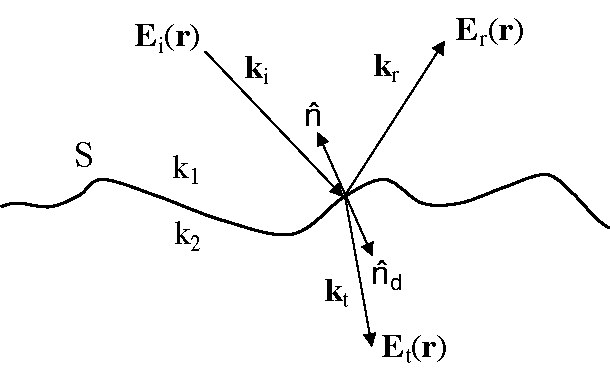
\includegraphics[width=2.5in]{Kirchhoff/Figures/kirchhoffgeometry} 
   \caption{Geometry for the Kirchhoff approximation at a dielectric interface}
     \label{kirchhoffgeo}
\end{figure}


In the far-field these simplify to
\begin{equation}
\G{1} \approx \left( \overline{\bb{I}} - \hat{k}_r \hat{k}_r \right) \dfrac{e^{ik_1r}}{4\pi r} \exp(-i \bb{k}_r \cdot \br') 
\end{equation}

\begin{equation}
\G{2} \approx \left( \overline{\bb{I}} - \hat{k}_t \hat{k}_t \right) \dfrac{e^{ik_2r}}{4\pi r} \exp(-i \bb{k}_t \cdot \br') 
\end{equation}

\noindent where $\bb{k}_r = k_1\hat{k}_r$ and $\bb{k}_t = k_2 \hat{k}_t$ are the reflected and transmitted wave vectors. The wave vectors are defined in the medium of propagation.  Substituting these
\begin{eqnarray}
\bb{E}_r(\br) & = & \dfrac{ik_1 e^{ik_1 r}}{4\pi r} \left( \overline{\bb{I}} - \hat{k}_r \hat{k}_r \right)  \int_S \left\{ \hat{k}_r \times \left[ \hat{n}' \times \bb{E}(\br')\right] + \eta_1\left[ \hat{n}' \times \bb{H}(\br')\right]\right\} e^{-i \bb{k}_r \cdot \br'} dS'   \\
\bb{E}_t(\br) & = & \dfrac{ik_2e^{ik_2r}}{4\pi r} \left( \overline{\bb{I}} - \hat{k}_t \hat{k}_t \right)  \int_S \left\{ \hat{k}_t \times \left[ \hat{n}_d' \times \bb{E}(\br')\right] + \eta_2\left[ \hat{n}_d' \times \bb{H}(\br')\right]\right\} e^{-i \bb{k}_t \cdot \br'}  dS'  
\end{eqnarray}

Next, define the orthonormal system $(\hat{p}_i,\hat{q}_i,\hat{k}_i)$ at point $\br'$ 
\begin{eqnarray}
\hat{q}_i &=& \dfrac{\hat{k}_i \times \hat{n} }{ \vert \hat{k}_i \times \hat{n} \vert } \\
\hat{p}_i &=& \hat{q}_i \times \hat{k}_i 
\end{eqnarray}

\noindent where $\hat{n}(\br') = -\hat{n}_d(\br')$.  Under the Kirchhoff approximation, the tangential electric and magnetic files for TE and TM fields are given by \eqref{ncrosse1} and \eqref{ncrosse2}, \cite{kong1986electromagnetic}, 
\begin{eqnarray}
\hat{n} \times \bb{E}(\br') & = & E_o\left\{ (\hat{e}_i \cdot \hat{q}_i )(\hat{n} \times \hat{q}_i) (1 + R^{\textrm{TE}}) + 
(\hat{e}_i \cdot \hat{p}_i )(\hat{n} \cdot \hat{k}_i) \hat{q}_i (1 - R^{\textrm{TM}}) \right\} e^{i\bb{k}_i \cdot \br'} \label{ncrosse1}  \\
\hat{n} \times \bb{H}(\br') & = & \dfrac{E_o}{\eta_1}\left\{ -(\hat{e}_i \cdot \hat{q}_i )(\hat{n} \cdot \hat{k}_i) \hat{q}_i (1 - R^{\textrm{TE}}) + (\hat{e}_i \cdot \hat{p}_i )(\hat{n} \times \hat{q}_i) (1 + R^{\textrm{TM}}) \right\} e^{i\bb{k}_i \cdot \br'}  \label{ncrosse2}
\end{eqnarray}

\noindent where $R^{\textrm{TE}}$ and $R^{\textrm{TM}}$ are the Fresnel reflection coefficients given in Section \ref{fresenlref}. The local incidence angle is
\eq{\cos\theta_i = -\hat{n} \cdot \hat{k}_i \label{localinctheta} }

Substituting these into the surface integral equations
\begin{eqnarray}
\bb{E}_r(\br) & = & \dfrac{ik_1e^{ik_1r}}{4\pi r} E_o \left( \overline{\bb{I}} - \hat{k}_r \hat{k}_r \right)  \cdot \int_S  \bb{F}(\br') e^{i (\bb{k}_i - \bb{k}_r) \cdot \br'} dS' \label{kirchint1} \\
\bb{E}_t(\br) & = & -\dfrac{ik_2e^{ik_2r}}{4\pi r} E_o \left( \overline{\bb{I}} - \hat{k}_t \hat{k}_t \right)  \cdot \int_S  \bb{N}(\br') e^{i (\bb{k}_i - \bb{k}_t) \cdot \br'} dS' \label{kirchint2} 
\end{eqnarray}

\noindent where
\begin{eqnarray}
\bb{F}(\br') &=&  - (\hat{e}_i \cdot \hat{q}_i )(\hat{n} \cdot \hat{k}_i) \hat{q}_i (1 - R^{\textrm{TE}}) + (\hat{e}_i \cdot \hat{p}_i )(\hat{n} \times \hat{q}_i) (1 + R^{\textrm{TM}}) \nonumber \\
\ & \ &+ (\hat{e}_i \cdot \hat{q}_i )(\hat{k}_r \times (\hat{n} \times \hat{q}_i)) (1 + R^{\textrm{TE}})  + (\hat{e}_i \cdot \hat{p}_i )(\hat{n} \cdot \hat{k}_i) (\hat{k}_r \times \hat{q}_i) (1 - R^{\textrm{TM}}) \\
\bb{N}(\br') &=&  - \dfrac{\eta_2}{\eta_1}(\hat{e}_i \cdot \hat{q}_i )(\hat{n} \cdot \hat{k}_i) \hat{q}_i (1 - R^{\textrm{TE}}) + \dfrac{\eta_2}{\eta_1}(\hat{e}_i \cdot \hat{p}_i )(\hat{n} \times \hat{q}_i) (1 + R^{\textrm{TM}}) \nonumber \\
\ & \ &+ (\hat{e}_i \cdot \hat{q}_i )(\hat{k}_t \times (\hat{n} \times \hat{q}_i)) (1 + R^{\textrm{TE}}) + (\hat{e}_i \cdot \hat{p}_i )(\hat{n} \cdot \hat{k}_i) (\hat{k}_t \times \hat{q}_i) (1 - R^{\textrm{TM}}) 
\end{eqnarray}

$\bb{F}$ and $\bb{N}$ only differ in the constants and wave vectors.  Due to the plane-wave approximation at the surface, the surface curvature must be large enough so that the Kirchhoff approximation is valid. Whether this is met or not, there are a number of ways to compute the integral depending on the application. One way is to finely discretize the surface at step sizes much smaller than the wavelength ($dS<\lambda/10$).  

\section{Fresnel Reflection Coefficients}
\label{fresenlref}
The Fresnel reflection coefficients for flat interfaces are given by, \cite{kong1986electromagnetic},
\begin{eqnarray}
R^{\textrm{TE}} &=& \dfrac{ \cos \theta_i - \sqrt{(\epsilon_2/\epsilon_1) - \sin^2\theta_i }}{\cos \theta_i + \sqrt{(\epsilon_2/\epsilon_1) - \sin^2\theta_i }} \\
R^{\textrm{TM}} &=& \dfrac{(\epsilon_2/\epsilon_1) \cos \theta_i - \sqrt{(\epsilon_2/\epsilon_1) - \sin^2\theta_i }}{(\epsilon_2/\epsilon_1) \cos \theta_i + \sqrt{(\epsilon_2/\epsilon_1) - \sin^2\theta_i }} 
\end{eqnarray}

The transmission coefficients are $T^{\textrm{TE}} = 1 + R^{\textrm{TE}}$ and $T^{\textrm{TM}} = 1 + R^{\textrm{TM}} $. In \cite{ulaby1999fundamentals}, there is a negative sign in the reflection coefficients that does not appear in \cite{kong1986electromagnetic}. This is due to the sign convention of incoming/outgoing field components. In \cite{kong1986electromagnetic}, the incoming and outgoing fields are defined relative to the $p$, $q$ coordinate projection, while in \cite{ulaby1999fundamentals} they are defined relative to incoming and outgoing plane wave directions, which flips the sign of $E$ and $H$ fields on reflection.  

The routines \texttt{fresnelTE} and \texttt{fresnelTM} compute the Fresnel reflection coefficients given the dielectric constants on either side of an interface, which can be complex, and the incidence angle in degrees.

{\footnotesize
\VerbatimInput{\code/Kirchhoff/fresnelTE.m}
}

{\footnotesize
\VerbatimInput{\code/Kirchhoff/fresnelTM.m}
}


%
%\section{Continuous Surfaces}
%
%One way to compute the integral is to finely discretize the surface and internal and perform the sum.  This is ultimately the most accurate.  It does however prevent simulating very large surfaces.  The surface curvature also demands attention, so that it stays in the range of validity of the Kirchhoff approximation. 
%

\section{Facetized Surfaces}

One way to compute equations \eqref{kirchint1} and \eqref{kirchint2} is to break up a large surface into many flat facets and compute the surface integrals analytically over the shapes of the facets. Discretizing the surface integral as a sum over large facets we have
\begin{eqnarray}
\bb{E}_r(\br) & \approx & \dfrac{ik_1e^{ik_1r}}{4\pi r} E_o \left( \overline{\bb{I}} - \hat{k}_r \hat{k}_r \right)  \cdot \sum_n \bb{F}(\br_n) \int_{S_n} e^{i (\bb{k}_i - \bb{k}_r) \cdot \br} dS \label{faceter} \\
\bb{E}_t(\br) & \approx & -\dfrac{ik_2e^{ik_2r}}{4\pi r} E_o \left( \overline{\bb{I}} - \hat{k}_t \hat{k}_t \right)  \cdot \sum_n \bb{N}(\br_n) \int_{S_n}  e^{i (\bb{k}_i - \bb{k}_t) \cdot \br} dS  \label{facetet}
\end{eqnarray}

\noindent where $S_n$ is the surface of the $n$th facet.  This assumes $\bb{F}(\br)$ and $\bb{N}(\br)$ are constant over the facet, i.e., the facet is flat and illuminated with plane waves. We are left with having to compute the surface phase integral over different facet shapes which can be written compactly in terms of the wave vector difference, $\bb{K}$, as
\eq{I = \int_S  e^{i\bb{K}\cdot \bb{r} } dS  \label{surfphaseint}}

\noindent where $\bb{K} = \bb{k}_i - \bb{k}_r$ or $\bb{K} = \bb{k}_i - \bb{k}_t$.  The surface phase integral is the 2D Fourier transform over the shape of the facet in the wave vector difference domain. 


\section{Surface Phase Integral}
\label{secsurfphaseint}
The surface phase integral is the 2D Fourier transform of the shape of a flat facet into the wave vector difference domain. Here we derive analytic expressions for the surface phase integral for common facet shapes. These will be used to derive closed-form expressions for the specular and backscatter RCS of PEC facets for these shapes.  The surface phase integral is given by 
\eq{I = \int_S  e^{i\bb{K}\cdot \bb{r} } dS  \label{surfphaseint2}}

\noindent where 
\ea{\bb{K} &=& \bb{k}_i - \bb{k}_s\\
 \bb{k}_i &=& k_i\left(\sin\theta_i \cos\phi_i \hat{x}  + \sin\theta_i \sin\phi_i \hat{y} + \cos\theta_i \hat{z}\right) \\
\bb{k}_s &=& k_s\left(\sin\theta_s \cos\phi_s \hat{x}  + \sin\theta_s \sin\phi_s \hat{y} + \cos\theta_s \hat{z}\right) \\
\bb{r}  &=& x \hat{x} + y \hat{y} + z \hat{z}}

The scattered wave vector, $\bb{k}_s$, can be a reflected or transmitted wave. If a facet is embedded in a large surface interface, the wavenumbers of the incident and scattered directions must correspond to correct medium above or below the interface. 

The surface phase integral can be computed for facets that are tilted arbitrarily in a global frame. However, analytic expressions are more easily derived using facets in the $XY$ plane, Figure \ref{kirchhoffXY}, which is our approach in the following subsections. When a facet is tilted in the global frame, the incident and scattered angles need to be transformed to the local frame of the facet. This can be done by first having the forward rotation of the facet relative to the global frame, then applying the rotation in reverse to the incident and scattered wave vectors in the global frame, which will give the incident and scattered wave vectors in the facet frame.

\begin{figure}[H] 
   \centering
   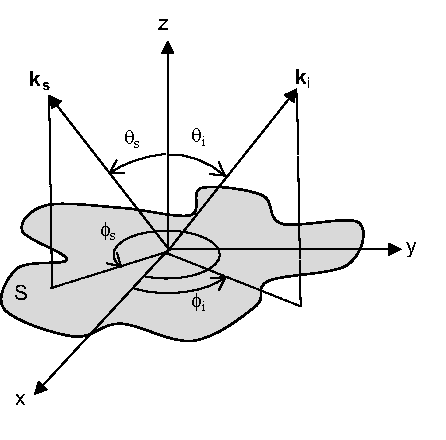
\includegraphics[width=2.5in]{Kirchhoff/Figures/surfacephaseint} 
   \caption{Geometry for the surface phase integral of a facet in the XY plane.}
     \label{kirchhoffXY}
\end{figure}




\addtocontents{toc}{\protect\setcounter{tocdepth}{1}}
\subsection{Specular Direction}
\addtocontents{toc}{\protect\setcounter{tocdepth}{2}}

Let the facet be in the $XY$ plane with $\hat{n} = \hat{z}$.  In the specular direction, $\theta_s = \pi - \theta_i$ and $\phi_s = \phi_i$, which means that the scattered direction is equivalent to the incident direction with the opposite $z$ component. The wave vector difference is then
\eq{\bb{k}_i - \bb{k}_s = 2 \cos\theta_i \hat{z}}

The position vector in this case is $\bb{r}  = x \hat{x} + y \hat{y}$.  Therefore, $(\bb{k}_i - \bb{k}_s)\cdot \bb{r} = 0$, so the complex exponent evaluates to one, and 
\eq{I = \int_S 1 \ dS = A}

\noindent where $A$ is the area of the facet. The surface phase integral in the specular direction is equal to the area of the facet. This is true for any shape.


\addtocontents{toc}{\protect\setcounter{tocdepth}{1}}
\subsection{Rectangle}
\addtocontents{toc}{\protect\setcounter{tocdepth}{2}}

Let a rectangular facet lie in the $XY$ plane with side lengths $L_x$ and $L_y$, $\hat{n} = \hat{z}$, and the facet is centered at the origin. The surface phase integral is written 
\begin{eqnarray}
I &=& \int_{-L_y/2}^{L_y/2}  \int_{-L_x/2}^{L_x/2}  e^{i\bb{K}\cdot \bb{r}} dx dy \\
\bb{K} &=& K_x \hat{x} + K_y \hat{y} + K_z \hat{z} \\
\bb{r} &=& x \hat{x} + y \hat{y}
\end{eqnarray}

\noindent where $\bb{K} = \bb{k}_i - \bb{k}_s$. The integral separates as 
\begin{eqnarray}
I &=& \int_{-L_x/2}^{L_x/2}  e^{i K_x x} dx  \int_{-L_y/2}^{L_y/2} e^{i K_y y} dy  \\
\end{eqnarray}

Using the fact that 
\eq{\int_{-a/2}^{a/2} e^{i b z} dz = \dfrac{2}{b} \sin\left(\dfrac{ab}{2}\right) }

and multiplying top and bottom by $L_xL_y$ to convert the sines to sinc functions, the surface phase integral over a rectangular facet is 
\eq{I = L_x L_y \textrm{sinc}\left(\dfrac{L_x K_x}{2}\right)\textrm{sinc}\left(\dfrac{L_y K_y}{2}\right) \label{SPIrect}}

%\ea{I &=& \dfrac{4}{K_x K_y} \sin\left(\dfrac{L_x K_x}{2}\right)\sin\left(\dfrac{L_y K_y}{2}\right) \\
%\ & = & L_x L_y \textrm{sinc}\left(\dfrac{L_x K_x}{2}\right)\textrm{sinc}\left(\dfrac{L_y K_y}{2}\right) }

\noindent where $\textrm{sinc}(x) = \sin(x)/x$. This is equal to the area of the facet multiplied by a directionally dependent function that has maximum value of one.




\addtocontents{toc}{\protect\setcounter{tocdepth}{1}}
\subsection{Ellipse}
\addtocontents{toc}{\protect\setcounter{tocdepth}{2}}

%Here we derive the analytic expression for the surface phase integral over an elliptical facet. 

Let the facet be an ellipse in the $XY$ plane centered at the origin such that $\hat{n} = \hat{z}$ with semi-major axis $a$ along the $x$ axis, and semi-minor axis $b$ along the $y$ axis, with a contour described by the equation
\eq{\dfrac{x^2}{a^2} + \dfrac{y^2}{b^2} = 1}

Using the change of variables
\ea{x &=& a \rho \cos\phi \\
y &=& b \rho \sin\phi \\
dS &=& a b \rho d\rho d\phi \\
\bb{r} &=&  a \rho \cos\phi \hat{x} + b \rho \sin\phi \hat{y} }

we transform \eqref{surfphaseint2} to an integration in polar coordinates over the surface of the ellipse as 
\eq{I = a b \int_0^{2\pi} \int_0^1 e^{i(K_x a \rho \cos\phi  + K_y b \rho \sin\phi)}  \rho d\rho d\phi }

Applying the following identity
\eq{\int_0^{2\pi} e^{ u \cos t +v \sin t} dt = 2 \pi I_0 \left( \sqrt{u^2 + v^2} \right)}

we get
\ea{I &=&  2 \pi  a b \int_{0}^{1}I_0 \left(i \rho \sqrt{  (a K_x)^2 + (b K_y)^2} \right) \rho d\rho  }

Finally, using
\eq{\int_0^1 I_0\left( i c x \right) x dx = \dfrac{J_1(c)}{c} }

the surface phase integral over an ellipse is
\ea{I &=&  2 \pi  a b \dfrac{J_1(K_{\rho}') }{K_{\rho}'} \\
\ &=& 2 \pi  a b \textrm{jinc}( K_{\rho}') \label{SPIellipse} \\
K_{\rho}' &=&  \sqrt{  (a K_x)^2 + (b K_y)^2} }

Note, $\textrm{jinc(0)} = 1/2$, so the final result is equal to the area of the ellipse multiplied by a directionally dependent term that has maximum value of one. $K_{\rho}'$ is a modified perpendicular component of the wave vector difference.  


\addtocontents{toc}{\protect\setcounter{tocdepth}{1}}
\subsection{Circle}
\addtocontents{toc}{\protect\setcounter{tocdepth}{2}}

The surface phase integral for the circular disk in the $XY$ plane with radius $a$ can be derived directly from the elliptical disk, \eqref{SPIellipse}, by taking $b = a$.  This gives
\ea{I &=&  2 \pi  a^2  \textrm{jinc}\left(a K_{\rho} \right) \label{SPIcircle} \\
K_{\rho} &=&  \sqrt{K_x ^2 +  K_y ^2}}

A solution for the circular disk can also be found in \cite{trott1988disk}, which uses a sequence of trigonometric transformations to separate the magnitude and phase of the perpendicular wave vector difference. %While it is possible to adapt that approach for an ellipse, it is easier to derive this using the wave vector difference, $\bb{K}$.  

\addtocontents{toc}{\protect\setcounter{tocdepth}{1}}
\subsection{Triangle}
\addtocontents{toc}{\protect\setcounter{tocdepth}{2}}

Let the facet be a triangle in the $XY$ plane with $\hat{n} = \hat{z}$. The vertices of the triangle are at positions $[\bb{p}_1, \bb{p}_2, \bb{p}_3]$. The vector to the triangle centroid is given by 
\eq{\br_n = \dfrac{1}{3}\left[\bb{p}_1+ \bb{p}_2+ \bb{p}_3\right] }

The phase integral is computed by mapping the domain of the arbitrary triangular facet to a triangle that covers half of the unit square though the following transform, \cite{triangleint},
\begin{eqnarray}
x(u,v) &=& x_1 + u(x_2 - x_1) + v(x_3 - x_1) \\
y(u,v) &=& y_1 + u(y_2 - y_1) + v(y_3 - y_1)  
\end{eqnarray}

\noindent where $u = [0,1]$ and $v = [0,1-u]$.  $\bb{p}_1$ is mapped to the origin, $\bb{p}_2$ is mapped to $(1,0)$ and $\bb{p}_3$ is mapped to $(0,1)$. The position vector is parameterized in terms of $u$ and $v$ as 
\eq{\bb{r}= \bb{p}_1 + u (\bb{p}_2 - \bb{p}_1) + v (\bb{p}_3 - \bb{p}_1) }

The change of variables in the surface integral is
\eq{I = \int_S f(x(u,v),y(u,v)) \vert \bb{J}(u,v)\vert du dv }

The determinant of the Jacobian is
\ea{\vert \bb{J}(u,v) \vert &=& \textrm{det} \twobytwo{\partial x /\partial u}{\partial x /\partial v}{\partial y /\partial u}{\partial y /\partial v} \\
\ & = & (x_2 - x_1)(y_3 - y_1) - (x_3 - x_1)(y_2 - y_1) \\
\ & = & 2 A
}
which is equal to the twice the area of the triangle.  With these, the integral becomes 
\eq{ I = 2 A \int_0^1\int_0^{1-u} e^{i(a + b u + c v)} dv du }

\noindent where 
\begin{eqnarray}
a &= & \bb{K} \cdot \bb{p}_1 \\ 
b &=& \bb{K} \cdot (\bb{p}_2 - \bb{p}_1)\\
c &=& \bb{K} \cdot (\bb{p}_3 - \bb{p}_1) 
\end{eqnarray}

Integrating this yields 
\ea{ I(a,b,c) &=& A e^{ia} g(b,c) \label{SPItriangle} \\
g(b,c) &=& 2 \dfrac{c(1 - e^{i b}) - b (1 - e^{ic})}{bc(b-c)}}

Divide by zero occurs for $b = 0$, $c = 0$, or $b = c$. The first two cases happen when the wave vector difference is perpendicular to an edge of the triangle. The third happens when the wave vector difference bisects the angle formed by two of the edges with $\bb{p}_1$ at the vertex.  The limits, though, exist and are given by 
\begin{eqnarray}
\lim_{b \rightarrow 0} g(b,c) &=& 2 \dfrac{1 + ic - e^{ic} }{c^2} \\
\lim_{c \rightarrow 0} g(b,c) &=& 2 \dfrac{1 + ib -e^{ib}}{b^2} \\
\lim_{c \rightarrow b} g(b,c) &=& 2 \dfrac{-1 +(1-ib) e^{ib}}{b^2} \\
\lim_{[b,c] \rightarrow [0,0]}g(b,c) &=& 1
\end{eqnarray}

%Assuming $\bb{K}$ is real, the magnitude squared of the auxiliary function is
%\ea{\vert g(b,c) \vert^2 &=& \dfrac{\left( c - c e^{i b} - b + b e^{ic}\right)\left( c - ce^{-i b} - b + b e^{-ic}\right)}{b^2c^2(b-c)^2} \\
%\ & =& b^2 \sin^2(c) + b^2 \cos^2(c) - 2 b^2 \cos(c) + b^2 + c^2 \sin^2(b) + c^2 \cos^2(b) - 2 c^2 \cos(b) - 2 b c - 2 b c \sin(b) \sin(c) + 2 b c \cos(b) + 2 b c \cos(c) - 2 b c \cos(b) \cos(c) + c^2 \\
%\ & =& 2 b^2 - 2 b^2 \cos(c)  + 2 c^2 - 2 b c  - 2 c^2 \cos(b)  + 2 b c \cos(b) + 2 b c \cos(c) - 2 b c (\sin(b) \sin(c)  + \cos(b) \cos(c)) \\
%\ & =& 2 b^2 (1-\cos(c))  + 2 c^2 (1 -  \cos(b)) - 2 b c  (1 - \cos(b) -  \cos(c)) - 2 b c \cos(b-c) \\
%\ & =& 2 b^2 (1-\cos(c))  + 2 c^2 (1 -  \cos(b)) - 2 b c  (1 - \cos(b) -  \cos(c) + \cos(b-c)) }

%\clearpage
%\newpage

\clearpage
\section{S-matrix of a Facet}

Here we develop the idea of an S-matrix for a Kirchhoff facet. The flat facet is treated as an isolated scatterer. When the facet is part of a larger surface discretization, the facet is assumed to be non-interacting with neighboring facets and which has homogeneous and semi-infinite mediums above and below it. We derive the general cases for the scattering of a facet and also provide expressions for their radar cross sections.


%Because of the preference of incident, scattered, and transmission depending on the medium with the originating wave, we can define four partially bistatic scattering quantities, $S_{11}$ and $S_{21}$, in which the incident field comes from medium 1 and reflects into medium 1 or transmits into medium 2, and $S_{12}$ and $S_{22}$ in which the incident field comes from medium 2.  $S_{11}$ and $S_{12}$ are defined above the interface, and $S_{21}$ and $S_{22}$ are defined below the interface.


Define the second orthonormal system $(\hat{p}_s,\hat{q}_s,\hat{k}_s)$ for the scattered field, which is relative to the surface of the facet and applies to both the reflected and transmitted fields, 
\begin{eqnarray}
\hat{q}_s &=& \dfrac{\hat{k}_s \times \hat{n} }{ \vert \hat{k}_s \times \hat{n} \vert } \\
\hat{p}_s &=& \hat{q}_s \times \hat{k}_s 
\end{eqnarray}

The unit vectors that make up the identity dyad are defined in terms of the scattered field system, $\overline{\bb{I}} = \hat{q}_s \hat{q}_s+ \hat{p}_s \hat{p}_s +\hat{k}_s \hat{k}_s$, so that the reflected and transmitted fields for a single facet are 
\begin{eqnarray}
\bb{E}_r(\br) & \approx & \dfrac{ik_1e^{ik_1r}}{4\pi r} E_o \left( \hat{q}_r \hat{q}_r+ \hat{p}_r \hat{p}_r \right)  \cdot  \bb{F}(\hat{k}_i,\hat{k}_r)  I(\bb{k}_i,\bb{k}_r) \\
\bb{E}_t(\br) & \approx & -\dfrac{ik_2e^{ik_2r}}{4\pi r} E_o \left( \hat{q}_t \hat{q}_t+ \hat{p}_t \hat{p}_t \right)  \cdot  \bb{N}(\hat{k}_i,\hat{k}_t)  I(\bb{k}_i,\bb{k}_t) 
\end{eqnarray}


\noindent where $I$ is the surface phase integral \eqref{surfphaseint}. 
Define two scattering matrices, $S_{11}$ and $S_{21}$, which map plane waves incident from medium 1 to far-field plane waves that are reflected or transmitted waves in mediums 1 and 2, respectively. $S_{11}$ is valid above the interface, while $S_{21}$ is valid below the interface.  Writing the incident, reflected and transmitted fields in the $\hat{p}$, $\hat{q}$ polarization basis
\begin{eqnarray}
\bb{E}_r & = & \dfrac{e^{ik_1r}}{r} \bb{S}_{11}  \cdot \bb{E}_i  \\
\bb{E}_t & = & \dfrac{e^{ik_2r}}{r} \bb{S}_{21}  \cdot \bb{E}_i  
\end{eqnarray}
\eq{\bb{E}_i  = E_o \twobyone{(\hat{e}_i \cdot \hat{p}_i )}{(\hat{e}_i \cdot \hat{q}_i )}}  

\noindent where the elements of the reflected and transmitted S-matrices are 
\ea{ \bb{S}_{11} &=& \dfrac{ik_1}{4\pi} I(\bb{k}_i,\bb{k}_r,\hat{n}) \tbt{\hat{p}_r \cdot \bb{F}_p }{\hat{p}_r \cdot \bb{F}_q }{\hat{q}_r \cdot \bb{F}_p }{\hat{q}_r \cdot \bb{F}_q} \label{S11kirch} }
\ea{ \bb{S}_{21} &=& -\dfrac{ik_2}{4\pi} I(\bb{k}_i,\bb{k}_t,\hat{n}) \tbt{\hat{p}_t \cdot \bb{N}_p }{\hat{p}_t \cdot \bb{N}_q }{\hat{q}_t \cdot \bb{N}_p }{\hat{q}_t \cdot \bb{N}_q} }

\noindent and
\ea{
\bb{F}_{p} &=&  (\hat{n} \times \hat{q}_i) (1 + R^{\textrm{TM}}) + (\hat{n} \cdot \hat{k}_i) (\hat{k}_r \times \hat{q}_i) (1 - R^{\textrm{TM}}) \\
\bb{F}_{q} &=& -(\hat{n} \cdot \hat{k}_i) \hat{q}_i (1 - R^{\textrm{TE}}) + (\hat{k}_r \times (\hat{n} \times \hat{q}_i)) (1 + R^{\textrm{TE}}) \\
\bb{N}_{p} &=& \dfrac{\eta_2}{\eta_1} (\hat{n} \times \hat{q}_i) (1 + R^{\textrm{TM}}) + (\hat{n} \cdot \hat{k}_i) (\hat{k}_t \times \hat{q}_i) (1 - R^{\textrm{TM}}) \\
\bb{N}_{q} &=& -\dfrac{\eta_2}{\eta_1} (\hat{n} \cdot \hat{k}_i) \hat{q}_i (1 - R^{\textrm{TE}}) + (\hat{k}_t \times (\hat{n} \times \hat{q}_i)) (1 + R^{\textrm{TE}}) }
%
%\ea{ \bb{F} &=&  \onebytwo{\bb{F}_{p}}{\bb{F}_{q}} \twobyone{(\hat{e}_i \cdot \hat{p}_i )}{(\hat{e}_i \cdot \hat{q}_i )}  \\
% \bb{N} &=&  \onebytwo{\bb{N}_{p}}{\bb{N}_{q}} \twobyone{(\hat{e}_i \cdot \hat{p}_i )}{(\hat{e}_i \cdot \hat{q}_i )} }

Table \ref{tableofdotproducts} gives the dot products between $\hat{p}$ and $\hat{q}$ and the different vector quantities listed at the top of the columns.
\begin{table}[htp]
\caption{Table of vector products}
\vspace{-3mm}
\begin{center}
\begin{tabular}{|c||c|c|c|c|}
\hline
& $\hat{n}\times\hat{q}_i$ & $\hat{k}\times\hat{q}_i$ & $\hat{q}_i$ & $\hat{k}\times(\hat{n}\times\hat{q}_i)$ \\ \hhline{|=|=|=|=|=|}
$\hat{p} \cdot$ & $\hat{n}\cdot (\hat{q}_i\times\hat{p}) $ & $-\hat{q}_i\cdot \hat{q}$  & $\hat{p}\cdot \hat{q}_i$ & $(\hat{k} \cdot \hat{q}_i) (\hat{p} \cdot \hat{n}) - (\hat{k} \cdot \hat{n}) (\hat{q}_i \cdot \hat{p}) $ \\ \hline
$\hat{q} \cdot$ & $\hat{n}\cdot (\hat{q}_i\times\hat{q}) $ & $\hat{p}\cdot \hat{q}_i$ &$ \hat{q} \cdot  \hat{q}_i$ & $ -(\hat{k} \cdot \hat{n}) (\hat{q} \cdot \hat{q}_i) $ \\ \hline
\end{tabular}
\end{center}
\label{tableofdotproducts}
\end{table}%

Using these, we can write
\ea{
\hat{p}_r \cdot \bb{F}_p & = & \hat{n}\cdot (\hat{q}_i\times\hat{p}_r) (1 + R^{\textrm{TM}}) + (\hat{n} \cdot \hat{k}_i) (-\hat{q}_i\cdot \hat{q}_r) (1 - R^{\textrm{TM}}) \label{prFp} \\ 
\hat{q}_r \cdot \bb{F}_p & = & \hat{n}\cdot (\hat{q}_i\times\hat{q}_r) (1 + R^{\textrm{TM}}) + (\hat{n} \cdot \hat{k}_i) (\hat{q}_i\cdot \hat{p}_r) (1 - R^{\textrm{TM}}) \\ 
\hat{p}_r \cdot \bb{F}_q & = & -(\hat{n} \cdot \hat{k}_i) (\hat{p}_r\cdot \hat{q}_i) (1 - R^{\textrm{TE}}) + ((\hat{k}_r \cdot \hat{q}_i) (\hat{p}_r \cdot \hat{n}) - (\hat{k}_r \cdot \hat{n}) (\hat{q}_i \cdot \hat{p}_r) ) (1 + R^{\textrm{TE}})  \\ 
\hat{q}_r \cdot \bb{F}_q & = &-(\hat{n} \cdot \hat{k}_i) (\hat{q}_r\cdot \hat{q}_i) (1 - R^{\textrm{TE}}) -(\hat{k}_r \cdot \hat{n}) (\hat{q}_r \cdot \hat{q}_i)  (1 + R^{\textrm{TE}})  \label{qrFq}
}

The same applies to $\bb{N}$ except with $r \rightarrow t$ and the inclusion of material constants. 

%
%Then we can write
%\ea{
%\hat{p}_s \cdot \bb{F}_p & = & \hat{n}\cdot (\hat{q}_i\times\hat{p}_s) (1 + R^{\textrm{TM}}) + (\hat{n} \cdot \hat{k}_i) (-\hat{q}_i\cdot \hat{q}_s) (1 - R^{\textrm{TM}})  \\ 
%\hat{q}_s \cdot \bb{F}_p & = & \hat{n}\cdot (\hat{q}_i\times\hat{q}_s) (1 + R^{\textrm{TM}}) + (\hat{n} \cdot \hat{k}_i) (\hat{q}_i\cdot \hat{p}_s) (1 - R^{\textrm{TM}}) \\ 
%\hat{p}_s \cdot \bb{F}_q & = & -(\hat{n} \cdot \hat{k}_i) (\hat{p}_s\cdot \hat{q}_i) (1 - R^{\textrm{TE}}) + ((\hat{k}_s \cdot \hat{q}_i) (\hat{p}_s \cdot \hat{n}) - (\hat{k}_s \cdot \hat{n}) (\hat{q}_i \cdot \hat{p}_s) ) (1 + R^{\textrm{TE}})  \\ 
%\hat{q}_s \cdot \bb{F}_q & = &-(\hat{n} \cdot \hat{k}_i) (\hat{q}_s\cdot \hat{q}_i) (1 - R^{\textrm{TE}}) -(\hat{k}_s \cdot \hat{n}) (\hat{q}_s \cdot \hat{q}_i)  (1 + R^{\textrm{TE}}) 
%}

%\clearpage
%\newpage
\section{Radar Cross Section of a Facet}


Recall that the polarized bistatic radar cross section is defined as
\ea{\sigma_{pq}(\hat{k}_s,\hat{k}_i) &=& \lim_{kr \rightarrow \infty} 4\pi r^2 \dfrac{\left\vert \hat{p} \cdot \bb{E}_s \right\vert^2}{\left\vert \hat{q} \cdot \bb{E}_i \right\vert^2} \\
\ &= & 4\pi \vert S_{pq} \vert^2 \label{Spq}}

The total radar cross section for either scattered polarization is \ea{\sigma_{p} &=& \sigma_{pp}(\hat{e}_i \cdot \hat{p}_i )^2 + \sigma_{pq}(\hat{e}_i \cdot \hat{q}_i )^2  \\
\sigma_{q} &=& \sigma_{qp}(\hat{e}_i \cdot \hat{p}_i )^2 + \sigma_{qq}(\hat{e}_i \cdot \hat{q}_i )^2  }

In the frame of the facet, $\hat{q}$ and $\hat{p}$ are equivalent to the traditional $\hat{h}$ and $\hat{v}$ polarizations.  In other words, if $\hat{n} = \hat{z}$, then $\hat{q}=\hat{h}$ and $\hat{p} = \hat{v}$ in a global frame.


\subsection{Specular RCS of a Facet}

The special case of the facet RCS in the specular direction can be derived using \eqref{S11kirch}.  Assume that the facet lies in the $XY$ plane with $\hat{n} = \hat{z}$. In the specular direction, we have $\theta_r = \pi - \theta_i$ and $\phi_r = \phi_i$, where the reflected wave vector is just the incidence wave vector reflected from the $XY$ plane. This means that
\ea{\hat{q}_r &=& \hat{q}_i \\
\hat{q}_i \cdot \hat{q}_r &=& 1 \\
\hat{p}_r \cdot \hat{q}_i &=& 0 \\
\hat{q}_i \times \hat{p}_r &=& -\hat{k}_r \\
\hat{q}_i \times \hat{q}_r &=& 0 \\
\hat{q}_i \times \hat{p}_r &=& 0}

Using these in \eqref{prFp}-\eqref{qrFq} gives:
\ea{\hat{p}_r \cdot \bb{F}_p & = & \hat{n}\cdot (-\hat{k}_r) (1 + R^{\textrm{TM}}) - (\hat{n} \cdot \hat{k}_i)  (1 - R^{\textrm{TM}})  \\ 
\hat{q}_r \cdot \bb{F}_p & = & 0 \\ 
\hat{p}_r \cdot \bb{F}_q & = &  0 \\ 
\hat{q}_r \cdot \bb{F}_q & = & -(\hat{n} \cdot \hat{k}_i) (1 - R^{\textrm{TE}}) - (\hat{k}_r\cdot \hat{n} )  (1 + R^{\textrm{TE}}) }

Using $\theta_i$ as the local incidence angle, we have for the specular direction $\cos\theta_i = -\hat{n} \cdot \hat{k}_i$ and $\cos\theta_i  = \hat{n} \cdot \hat{k}_r$. Substituting these and simplifying, we can write the polarized RCSs as
\ea{\sigma_{pp}  &=&  \sigma_{pec}\vert R^{\textrm{TM}} \vert^2 \\
\sigma_{qq}  &=&  \sigma_{pec}\vert R^{\textrm{TE}}\vert^2  }
\eq{\sigma_{pq} = \sigma_{qp} = 0}

\noindent where 
\eq{\sigma_{pec}  = \dfrac{k^2}{\pi} \cos^2\theta_i \vert I(\bb{k}_i,\bb{k}_r)\vert^2 \label{kapecspec} }

and $\sigma_{pec}$ is the RCS for a PEC surface, evaluated in the specular direction. This quantity assumes perfect reflection, and $\theta_i$ is the local incidence angle measured from the facet normal. These show that 1) there are no cross polarization terms for the specular direction of a flat facet under the Kirchhoff approximation, and 2) the specular RCS of a facet at a dielectric interface is the same as a PEC facet only scaled by the reflectivity of the surface evaluated at the incidence angle.  Derived above, the value of $\vert I\vert^2$ in the specular direction is equal to the area of the facet squared. This is true regardless of the shape. Therefore, in the specular direction, the RCS of a PEC facet is just 
\eq{\sigma_{pec}  = \dfrac{k^2}{\pi} \cos^2\theta_i A^2  \label{specRCS} }

\begin{table}[h]
\caption{Specular RCS of a PEC Facet}
\begin{center}
\begin{tabular}{|p{1.8cm}|p{3.2cm}|c|p{2.7cm}|}
\hline
Facet & Geometry & $\sigma_{pec}$ & Notes \\
\hline
Any shape & \parbox[c]{1em}{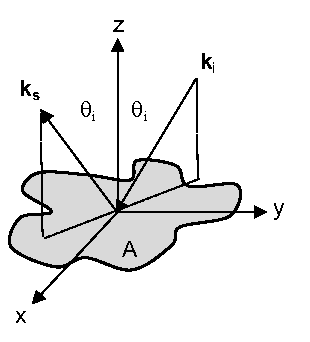
\includegraphics[width=1.2in]{Kirchhoff/Figures/Specular}}  & $\dfrac{k^2}{\pi} \cos^2\theta_i A^2$ & $A$ is the facet area \\   \hline
\end{tabular}
\label{tablePECspecRCS}
\end{center}
\end{table}


\subsection{Backscatter RCS of a Facet}

To obtain the backscatter RCS of a facet, we use \eqref{S11kirch} with $\hat{k}_r = -\hat{k}_i$, $\hat{q}_r = -\hat{q}_i$, $\hat{p}_r = \hat{p}_i$. Substituting these into \eqref{prFp}-\eqref{qrFq} it can be shown that 
\ea{
\hat{p}_r \cdot \bb{F}_p & = & -2(\hat{n}\cdot \hat{k}_i) R^{\textrm{TM}}  \\ 
\hat{q}_r \cdot \bb{F}_p & = & 0 \\ 
\hat{p}_r \cdot \bb{F}_q & = & 0 \\ 
\hat{q}_r \cdot \bb{F}_q & = & -2(\hat{n} \cdot \hat{k}_i)  R^{\textrm{TE}} 
}

Then using  \eqref{S11kirch} and \eqref{Spq}, we get
\ea{\sigma_{pp}  &=&  \sigma_{pec}\vert R^{\textrm{TM}} \vert^2 \\
\sigma_{qq}  &=&  \sigma_{pec}\vert R^{\textrm{TE}}\vert^2  }
\eq{\sigma_{pq} = \sigma_{qp} = 0}

where 
\eq{\sigma_{pec}  = \dfrac{k^2}{\pi} \cos^2\theta_i \vert I(\bb{k}_i,-\bb{k}_i)\vert^2 \label{kasigmapec} }

\noindent where $\sigma_{pec}$ is the backscatter RCS for a PEC surface. As with the specular direction, this assumes perfect reflection, and $\theta_i$ is the local incidence angle measured from the facet normal. There are no cross polarization terms for the backscatter of a flat facet under the Kirchhoff approximation, and the backscatter RCS of a facet at a dielectric interface is equal to the backscatter RCS of a PEC facet scaled by the reflectivity. The surface phase integral has to be evaluated over the facet shape. We use the results from Section \ref{secsurfphaseint} to find $\sigma_{pec}$ in the backscatter direction for simple shapes.

%%(-\hat{q}_i)
%%(-\hat{k}_i)
%\ea{
%\hat{p}_r \cdot \bb{F}_p & = & \hat{n}\cdot (\hat{q}_i\times\hat{p}_i) (1 + R^{\textrm{TM}}) + (\hat{n} \cdot \hat{k}_i) (-\hat{q}_i\cdot (-\hat{q}_i)) (1 - R^{\textrm{TM}})  \\ 
%\hat{q}_r \cdot \bb{F}_p & = & \hat{n}\cdot (\hat{q}_i\times(-\hat{q}_i)) (1 + R^{\textrm{TM}}) + (\hat{n} \cdot \hat{k}_i) (\hat{q}_i\cdot \hat{p}_i) (1 - R^{\textrm{TM}}) \\ 
%\hat{p}_r \cdot \bb{F}_q & = & -(\hat{n} \cdot \hat{k}_i) (\hat{p}_i\cdot \hat{q}_i) (1 - R^{\textrm{TE}}) + (((-\hat{k}_i) \cdot \hat{q}_i) (\hat{p}_i \cdot \hat{n}) - ((-\hat{k}_i)\cdot \hat{n}) (\hat{q}_i \cdot \hat{p}_i) ) (1 + R^{\textrm{TE}})  \\ 
%\hat{q}_r \cdot \bb{F}_q & = &-(\hat{n} \cdot \hat{k}_i) ((-\hat{q}_i)\cdot \hat{q}_i) (1 - R^{\textrm{TE}}) -((-\hat{k}_i) \cdot \hat{n}) ((-\hat{q}_i)\cdot \hat{q}_i)  (1 + R^{\textrm{TE}}) 
%}
%
%\ea{
%\hat{p}_r \cdot \bb{F}_p & = & \hat{n}\cdot (\hat{q}_i\times\hat{p}_i) (1 + R^{\textrm{TM}}) + (\hat{n} \cdot \hat{k}_i)  (1 - R^{\textrm{TM}})  \\ 
%\hat{q}_r \cdot \bb{F}_p & = & 0 \\ 
%\hat{p}_r \cdot \bb{F}_q & = & 0 \\ 
%\hat{q}_r \cdot \bb{F}_q & = & (\hat{n} \cdot \hat{k}_i)  (1 - R^{\textrm{TE}}) -(\hat{k}_i \cdot \hat{n})  (1 + R^{\textrm{TE}}) 
%}
%
%\ea{
%\hat{p}_r \cdot \bb{F}_p & = & -\hat{n}\cdot \hat{k}_i (1 + R^{\textrm{TM}}) + (\hat{n} \cdot \hat{k}_i)  (1 - R^{\textrm{TM}})  \\ 
%\hat{q}_r \cdot \bb{F}_p & = & 0 \\ 
%\hat{p}_r \cdot \bb{F}_q & = & 0 \\ 
%\hat{q}_r \cdot \bb{F}_q & = & (\hat{n} \cdot \hat{k}_i)  (1 - R^{\textrm{TE}}) -(\hat{k}_i \cdot \hat{n})  (1 + R^{\textrm{TE}}) 
%}



%
%The bi-static radar cross-section is defined 
%\eq{\sigma_{pq}(\hat{k}_s,\hat{k}_i) = \lim_{kr \rightarrow \infty} 4\pi r^2 \dfrac{\left\vert \hat{p} \cdot \bb{E}_s \right\vert^2}{\left\vert \hat{q} \cdot \bb{E}_i \right\vert^2} }
%
%(not the same pq as Kirchhoff derivation).  For a single object, the scattered field is 
%\begin{eqnarray}
%\bb{E}_s(\br) & \approx & \dfrac{ike^{ikr}}{4\pi r} E_o \left( \overline{\bb{I}} - \hat{k}_s \hat{k}_s \right)  \cdot  \bb{F} I \nonumber \\
%\end{eqnarray}
%
%For backscatter in the medium above the facet, $\hat{k}_r = -\hat{k}_i$, and using $\overline{\bb{I}} = \hat{q} \hat{q} + \hat{p} \hat{p} +\hat{k}_s \hat{k}_s$, the field is 
%\begin{eqnarray}
%\bb{E}_s(\br) & \approx & \dfrac{ike^{ikr}}{4\pi r} E_o \left( \hat{q} \hat{q} + \hat{p} \hat{p}\right)  \cdot  \bb{F} I \nonumber \\
%\end{eqnarray}
%
%where 
%\ea{\bb{F} &=&  - (\hat{e}_i \cdot \hat{q} )(\hat{n} \cdot \hat{k}_i) \hat{q} (1 - R^{\textrm{TE}}) + (\hat{e}_i \cdot \hat{p} )(\hat{n} \times \hat{q}) (1 + R^{\textrm{TM}}) \nonumber \\
%\ & \ &+ (\hat{e}_i \cdot \hat{q} )(-\hat{k}_i \times (\hat{n} \times \hat{q})) (1 + R^{\textrm{TE}}) + (\hat{e}_i \cdot \hat{p} )(\hat{n} \cdot \hat{k}_i) (-\hat{k}_i \times \hat{q}) (1 - R^{\textrm{TM}}) \nonumber \\}
%
%\ea{-\hat{k}_i \times (\hat{n} \times \hat{q}) &=& \hat{q}(\hat{n} \cdot \hat{k}_i) \\
%-\hat{k}_i \times \hat{q} &=& \hat{p} }
%
%so
%\ea{\bb{F} &=&  - (\hat{e}_i \cdot \hat{q} )(\hat{n} \cdot \hat{k}_i) \hat{q} (1 - R^{\textrm{TE}})  + (\hat{e}_i \cdot \hat{p} )(\hat{n} \times \hat{q}) (1 + R^{\textrm{TM}}) \nonumber \\
%\ & \ & + (\hat{e}_i \cdot \hat{q} )(\hat{n} \cdot \hat{k}_i)\hat{q} (1 + R^{\textrm{TE}}) \nonumber  + (\hat{e}_i \cdot \hat{p} )(\hat{n} \cdot \hat{k}_i) \hat{p}(1 - R^{\textrm{TM}}) }
%
%%or 
%%
%%\ea{\bb{F} &=&  - (\hat{e}_i \cdot \hat{q} )(\hat{n} \cdot \hat{k}_i)2 R^{\textrm{TE}}  \hat{q}\nonumber \\
%%\ & \ &  +  (\hat{e}_i \cdot \hat{p} ) \left(   (\hat{n} \times \hat{q}) (1 + R^{\textrm{TM}})  + (\hat{n} \cdot \hat{k}_i) \hat{p}(1 - R^{\textrm{TM}}) \right) }
%
%
%The scattered field is 
%\begin{eqnarray}
%\bb{E}_s & \approx & \dfrac{ike^{ikr}}{4\pi r} E_o \left( F_q \hat{q} + F_p \hat{p}\right)  I \nonumber \\
%\end{eqnarray}
%
%%with 
%
%\ea{F_q &=& - (\hat{e}_i \cdot \hat{q} )(\hat{n} \cdot \hat{k}_i)2 R^{\textrm{TE}}  \\
%F_p &=&   (\hat{e}_i \cdot \hat{p} ) \left(  \hat{p}\cdot (\hat{n} \times \hat{q}) (1 + R^{\textrm{TM}})  + (\hat{n} \cdot \hat{k}_i) (1 - R^{\textrm{TM}}) \right) }
%
%using $\hat{p}\cdot (\hat{n} \times \hat{q}) = -\hat{p} (\hat{n} \cdot \hat{k}_i) $ and $(\hat{n} \cdot \hat{k}_i) = -\cos\theta_i$ this is equal to 
%\ea{F_q &=&  (\hat{e}_i \cdot \hat{q} ) 2 \cos\theta_i R^{\textrm{TE}}   \\
%F_p &=&   (\hat{e}_i \cdot \hat{p} ) \left(  \cos\theta_i  (1 + R^{\textrm{TM}})  -\cos\theta_i (1 - R^{\textrm{TM}}) \right) }
%
%or
%\ea{F_q &=&  (\hat{e}_i \cdot \hat{q} ) 2 \cos\theta_i R^{\textrm{TE}}   \\
%F_p &=&   (\hat{e}_i \cdot \hat{p} ) 2 \cos\theta_i R^{\textrm{TM}} }
%
%
%The scattered power is 
%\begin{eqnarray}
%\vert \bb{E}_s \vert^2 & = & \dfrac{k^2}{(4\pi)^2 r^2} \vert E_o\vert^2 \left(  \vert F_q \vert^2 +  \vert F_p \vert^2 \right)  I^2 \nonumber \\
%\end{eqnarray}
%
%The incident field and power are  
%\eq{ \bb{E}_i = E_o ((\hat{e}_i \cdot \hat{q} ) \hat{q} + (\hat{e}_i \cdot \hat{p} ) \hat{p} )}
%\eq{\vert \bb{E}_i \vert^2 = \vert E_o\vert^2 }
%
%The total cross-section is defined 
%\eq{\sigma = \lim_{kr \rightarrow \infty} 4\pi r^2 \dfrac{\left\vert \bb{E}_s \right\vert^2}{\left\vert \bb{E}_i \right\vert^2} }
%
%Then the total backscatter is 
%\ea{\sigma &=& \dfrac{k^2}{4\pi} \left(  \vert F_q \vert^2 +  \vert F_p \vert^2 \right)  I^2  }
%
%and substituting and equating $\hat{h} = \hat{q}$ and $\hat{v} = \hat{p}$, 
%\ea{\sigma &= & \sigma_{hh} (\hat{e}_i \cdot \hat{h} )^2 + \sigma_{vv}(\hat{e}_i \cdot \hat{v} ) ^2 }
%
%\noindent where
%\ea{\sigma_{hh}  =  \sigma_{pec}\vert R^{\textrm{TE}}\vert^2  \\
%\sigma_{vv}  =  \sigma_{pec}\vert R^{\textrm{TM}} \vert^2 }
%
%and
%\eq{\sigma_{pec}  = \dfrac{k^2}{\pi} \cos^2\theta_i I^2 }
%
%depends on the shape of the surface.


%
%\subsection{Local bistatic scattering angles}
%
%So far the $\hat{p}$ and $\hat{q}$ polarization decomposition is relative to the facet normal. We need to relate bistatic angles in a global frame to those in the frame of the facet to help with evaluating the surface phase integral.  \cite{van2011synthetic} and Tsang give such transforms for problems with cylindrical symmetry. In general, we want to transform between  
%
%Define the generic incident 
%\ea{ \hat{k}_i &=& \sin\theta_i \cos\phi_i \hat{x}  + \sin\theta_i \sin\phi_i \hat{y} + \cos\theta_i \hat{z}  \\
%\hat{k}_s &=& \sin\theta_s \cos\phi_s \hat{x}  + \sin\theta_s \sin\phi_s \hat{y} + \cos\theta_s \hat{z}  }
%
%The local incident angle for use in the reflection coefficients is  
%\eq{\cos\theta_{i} = -\hat{n} \cdot \hat{k}_i }
%
%The relative incident and scattered angles used in the surface phase integral when its normal is in the $+z$ are (following the notation in [van Zyl])
%\eq{\cos\theta_{ic} = \hat{n} \cdot \hat{k}_i }
%\eq{\cos\theta_{sc} = \hat{n} \cdot \hat{k}_s }
%
%Defining   
%\ea{ \hat{n} &=& \sin\theta_c \cos\phi_c \hat{x}  + \sin\theta_c \sin\phi_c \hat{y} + \cos\theta_c \hat{z}  }
%
%\noindent where $(\theta_c,\phi_c)$ are the spherical angles of the normal vector.  Finally, we can find the relative azimuth angles $\phi_{ic} = \phi_c - \phi_i$ and $\phi_{sc} = \phi_c - \phi_s$ from 
%\ea{\hat{n} \cdot \hat{k}_i &=&  \cos\theta_c\cos\theta_i + \sin\theta_c\sin\theta_i \cos(\phi_c - \phi_i) \\
%\hat{n} \cdot \hat{k}_s &=&  \cos\theta_c\cos\theta_s + \sin\theta_c\sin\theta_s \cos(\phi_c - \phi_s) }
%





%
%\ea{
%\hat{p}_s \cdot \bb{F}_p & = & -\cos\theta_i (1 + R^{\textrm{TM}}) +\cos\theta_i  (1 - R^{\textrm{TM}})  \\ 
%\hat{q}_s \cdot \bb{F}_q & = & \cos\theta_i  (1 - R^{\textrm{TE}}) -\cos\theta_i  (1 + R^{\textrm{TE}}) 
%}
%\ea{
%\hat{p}_s \cdot \bb{F}_p & = & -2 \cos\theta_i  R^{\textrm{TM}}  \\ 
%\hat{q}_s \cdot \bb{F}_q & = & -2\cos\theta_i   R^{\textrm{TE}} 
%}
%
%Therefore, the specular cross sections are 
%\ea{\sigma_{hh} &=& 4\pi \vert S_{hh} \vert^2 \\
%\ &=&  4 \pi \dfrac{k^2}{(4\pi)^2} \vert I \vert^2 \vert \hat{q}_s \cdot \bb{F}_q  \vert^2 \\
%\ &= & \dfrac{k^2}{\pi} \cos^2\theta_i \vert R^{\textrm{TE}} \vert^2 \vert I \vert^2 }
%
%Likewise for $vv$.  Or 
%\ea{\sigma_{hh}  =  \sigma_{pec}\vert R^{\textrm{TE}}\vert^2  \\
%\sigma_{vv}  =  \sigma_{pec}\vert R^{\textrm{TM}} \vert^2 }
%
%and
%\eq{\sigma_{pec}  = \dfrac{k^2}{\pi} \cos^2\theta_i I^2 }
%
%In all the cases below, the value of the $I^2$ for the specular direction is just the area of the surface squared, so that
%
%\eq{\sigma_{pec}  = \dfrac{k^2}{\pi} \cos^2\theta_i A^2  }

%
%\subsection{Forward Cross Section}
%
%This is the scattering through an interface of a finite area.

\paragraph{Rectangle} Assuming that the facet is in the $XY$ plane with $\hat{n} = \hat{z}$. In the backscatter direction $k_i = k_s = k$, $\theta_s = \pi - \theta_i$ and $\phi_s = \phi_i + \pi$, and it can be shown that the components of the wave vector difference is equal to 
\ea{K_x &=& 2 k \sin\theta_i \cos\phi_i \label{Kxback} \\
K_y &=& 2 k \sin\theta_i \sin\phi_i \label{Kyback} }

The surface phase integral in over a rectangle, \eqref{SPIrect}, in the backscatter direction is 
\eq{I = L_x L_y \textrm{sinc}\left(L_x k \sin\theta_i \cos\phi_i\right)\textrm{sinc}\left(L_y k \sin\theta_i \sin\phi_i\right)}

Using this in \eqref{kasigmapec}, the backscatter RCS of a  rectangular PEC facet is 
\eq{\sigma_{pec}  = \dfrac{k^2}{\pi} \cos^2\theta_i L_x^2 L_y^2 \textrm{sinc}^2\left(L_x k \sin\theta_i \cos\phi_i\right)\textrm{sinc}^2\left(L_y k \sin\theta_i \sin\phi_i\right) }
 
In \eqref{kasigmapec}, $\cos\theta_i$ was defined for the local incident angle using \eqref{localinctheta}. However, the angles in the argument of the sinc technically belong to the incident wave vector. Because $\textrm{sinc}(x)$ is even, and because $\theta_i \rightarrow \pi - \theta_i$ and $\phi_i \rightarrow \phi_i + \pi$, the result is the same. Therefore, the angles can be treated as belonging to either the incident wave vector or a vector that points to the sensor for the case of backscatter. Note, the RCS is proportional to the area of the facet squared.

\paragraph{Ellipse} 
Assuming that the facet is in the $XY$ plane, and with \eqref{Kxback} and \eqref{Kyback}, the surface phase integral over an ellipse, \eqref{SPIellipse} reduces to 
\ea{I &=&  2 \pi  a b \textrm{jinc}\left( 2k\sin\theta_i  \sqrt{  a^2 \cos^2\phi_i  + b^2 \sin^2\phi_i  }\right) \label{SPIellipseback} }

Using this in the expression for radar cross section for a PEC surface, \eqref{kasigmapec}, the backscatter RCS of a PEC elliptical disk is  
 \eq{\sigma_{pec}  = 4 \pi k^2 \cos^2\theta_i a^2 b^2 \textrm{jinc}^2\left(2 k \sin\theta_i \sqrt{  a^2 \cos^2\phi_i  + b^2 \sin^2\phi_i  } \right) \label{pedbackscatterellipse} }
%
Because this is an even function of $\theta_i$ and $\phi_i$, the angles can be defined either from the incident wave vector or from a vector that points to the sensor and measured from the facet normal.  

\paragraph{Circle} Using \eqref{SPIellipseback} with $b=a$, the surface phase integral for a circular disk is
\ea{I &=&  2 \pi  a^2 \textrm{jinc}\left( 2k\sin\theta_i a \right)}

Likewise, from \eqref{pedbackscatterellipse}, the backscatter RCS of the circular PEC disk is
 \eq{\sigma_{pec}  = 4 \pi k^2 a^4 \cos^2\theta_i  \textrm{jinc}^2\left(2 k a \sin\theta_i \right)  }

Again, $\theta_i$ can be either the forward incident angle, or the local incident angle from facet normal.

\paragraph{Triangle} For the backscatter direction, $\bb{K} = 2 \bb{k}_i $. When $\bb{K}$ is real, the surface phase integral of a triangular facet, \eqref{SPItriangle}, has the following identity $I(-a,-b,-c) = I^*(a,b,c)$. Therefore, reversing the incident direction to use angles that point at the sensor will not change $\vert I \vert^2$. The backscatter RCS of a PEC triangle is then
\eq{\sigma_{pec}  = \dfrac{k^2}{\pi}  A^2 \cos^2\theta_i \vert g(b,c)\vert^2 }

No simple reduction has been found for $\vert g(b,c)\vert^2$. 

\paragraph{Summary}
Table \ref{tablePECbackRCS} has a summary of $\sigma_{pec}$ for these shapes. In general, $\sigma_{pec}$ can be decomposed as a product of four terms: 1) a factor of $k^2/\pi$, 2) a factor of $\cos^2\theta_i$ for the area projection, 3) a factor of the facet area, and 4) a directionally dependent weighting function that has maximum value of one and comes from the Fourier transform over the domain of the facet via the surface phase integral. 
%\clearpage
%\newpage
 
\begin{table}[h]
\caption{Backscatter RCS of PEC Facets}\label{tablePECbackRCS}
%\vspace{-1.5\baselineskip}
\begin{center}
\begin{tabular}{|p{1.6cm}|p{2.8cm}|c|p{2.9cm}|}
\hline
Facet & Geometry & $\sigma_{pec}$ & Notes \\
\hline
Any shape & \quad \parbox[c]{1em}{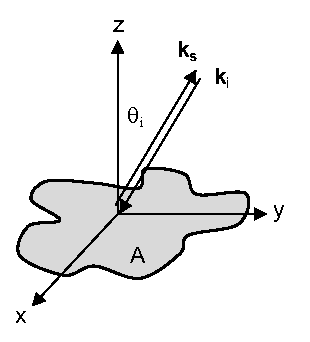
\includegraphics[width=1in]{Kirchhoff/Figures/Backscatter}}  &$\dfrac{k^2}{\pi} \cos^2\theta_i \vert I(\bb{k}_i,-\bb{k}_i)\vert^2 $ &  \\   \hline
Rectangle & \parbox[c]{1em}{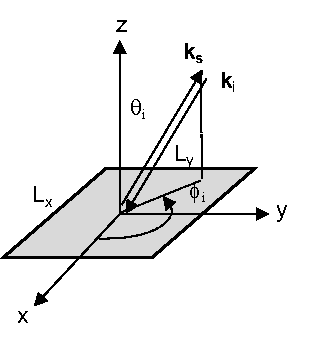
\includegraphics[width=1in]{Kirchhoff/Figures/Rectangle}}  & $\begin{array}{c} \dfrac{k^2}{\pi} \cos^2\theta_i L_x^2 L_y^2 \cdot \\ \textrm{sinc}^2\left(L_x k \sin\theta_i \cos\phi_i\right)\textrm{sinc}^2\left(L_y k \sin\theta_i \sin\phi_i\right) \end{array}$ & $\textrm{sinc}(x) = \dfrac{\sin(x)}{x}$ \\   \hline
Ellipse & \parbox[c]{1em}{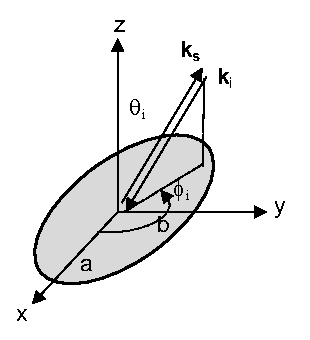
\includegraphics[width=1in]{Kirchhoff/Figures/Ellipse}}  & $\begin{array}{c} 4 \pi k^2 \cos^2\theta_i a^2 b^2 \cdot \\
\textrm{jinc}^2\left(2 k \sin\theta_i \sqrt{  a^2 \cos^2\phi_i  + b^2 \sin^2\phi_i  } \right) \end{array} $ & $\textrm{jinc}(x) = \dfrac{J_1(x) }{x} $ \\   \hline
Circle & \parbox[c]{1em}{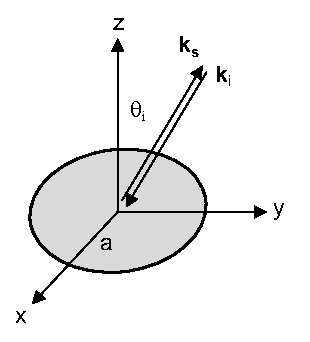
\includegraphics[width=1in]{Kirchhoff/Figures/Circle}}  &$ 4 \pi k^2 a^4 \cos^2\theta_i  \textrm{jinc}^2\left(2 k a \sin\theta_i \right)$  &  \\   \hline
Triangle & \parbox[c]{1em}{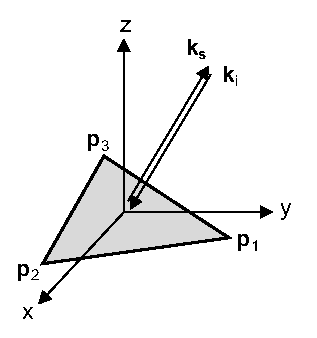
\includegraphics[width=1in]{Kirchhoff/Figures/Triangle}}  & $\dfrac{k^2}{\pi}  A^2 \cos^2\theta_i \vert g(b,c)\vert^2 $ & \footnotesize$\begin{array}{l}
b = \bb{K} \cdot (\bb{p}_2 - \bb{p}_1) \\
c = \bb{K} \cdot (\bb{p}_3 - \bb{p}_1) \\
%\dfrac{1}{3}\left[\bb{p}_1+\bb{p}_2+\bb{p}_3\right] = 0
\end{array}$ \\   \hline
\end{tabular}
\end{center}
\end{table}%
 


%2 \pi  a b \textrm{jinc}\left(\Omega \Gamma \right) }




%
%There are two approaches to this deviation. The first can be done in terms of the components $K_x$ and $K_y$. The second uses a sequence of trigonometric manipulations in order to separate the 
%
%Writing out the dot product and collecting like factors of $\sin\theta$
%\ea{
%  (\bb{k}_i - \bb{k}_s) \cdot  \bb{r} &=& a \rho \cos\phi (k_i \sin\theta_i \cos\phi_i - k_s\sin\theta_s \cos\phi_s )   + b \rho \sin\phi ( k_i \sin\theta_i \sin\phi_i  - k_s\sin\theta_s \sin\phi_s ) \nonumber \\
%\ & \ & \\
%\ &=& k_i \rho \sin\theta_i ( a \cos\phi \cos\phi_i + b \sin\phi \sin\phi_i ) - k_s \rho \sin\theta_s (a \cos\phi \cos\phi_s + b \sin\phi \sin\phi_s ) \nonumber \\ }
%
%Next, we use the identity 
%\ea{a \cos\alpha \cos\beta + b \sin\alpha \sin\beta  &=& \dfrac{1}{2}\left( (a + b) \cos(\alpha - \beta) + (a-b) \cos(\alpha + \beta) \right) }
%
%to convert the trigonometric products to cosines and then factor the sum and difference of the ellipse parameters 
%\ea{\ &=&  k_i \rho \sin\theta_i \dfrac{1}{2}\left( (a + b) \cos(\phi - \phi_i) + (a-b) \cos(\phi + \phi_i)\right)   \\ 
%\ & \ & - k_s \rho \sin\theta_s \dfrac{1}{2}\left( (a + b) \cos(\phi - \phi_s) + (a-b) \cos(\phi + \phi_s)\right) \\
%%&=&  k_i \rho \dfrac{1}{2}  \left( (a + b) \sin\theta_i \cos(\phi - \phi_i) + (a-b) \sin\theta_i \cos(\phi + \phi_i)\right)   \\ 
%%\ & \ & - k_s \rho  \dfrac{1}{2}\left( (a + b) \sin\theta_s\cos(\phi - \phi_s) + (a-b) \sin\theta_s\cos(\phi + \phi_s)\right) \\ 
%&=&  \rho \dfrac{1}{2} (a + b)  \left( k_i\sin\theta_i \cos(\phi - \phi_i) -  k_s\sin\theta_s\cos(\phi - \phi_s)\right)  \\
%\ & \ & + \rho \dfrac{1}{2}(a-b) \left(  k_i\sin\theta_i \cos(\phi + \phi_i) - k_s\sin\theta_s\cos(\phi + \phi_s) \right)  }
%
%Following \cite{trott1988disk}, the trick is to manipulate the sines and cosines in order to isolate $\phi$.  This starts by equating the terms in the parentheses to a phased cosine 
%\ea{k_i \sin\theta_i \cos(\phi \mp \phi_i) - k_s\sin\theta_s \cos(\phi \mp \phi_s) & =& \Omega_{\mp} \cos(\phi \mp \gamma) }
%
%Next, apply the sum/difference of angles formula
%\ea{\cos(\alpha \mp \beta) &=& \cos\alpha\cos\beta \pm \sin\alpha\sin\beta \\}
%
%to the left and right sides to get 
%\eq{k_i \sin\theta_i (\cos\phi\cos\phi_i \pm \sin\phi\sin\phi_i ) - k_s \sin\theta_s (\cos\phi\cos\phi_s \pm \sin\phi\sin\phi_s) = \Omega_{\mp} (\cos\phi\cos\gamma \pm \sin\phi\sin\gamma)    }
%
%Equating factors of $\cos\phi$ and $\sin\phi$, we have the relations
%\ea{\Omega_{\mp} \cos\gamma  &=& k_i \sin\theta_i \cos\phi_i- k_s \sin\theta_s\cos\phi_s \label{omega1} \\
%\pm \Omega_{\mp} \sin\gamma  &=& \pm k_i \sin\theta_i \sin\phi_i \mp k_s \sin\theta_s\sin\phi_s \label{omega2} \\
%\Omega_{\mp}^2  &=& (k_i \sin\theta_i \cos\phi_i- k_s \sin\theta_s\cos\phi_s)^2 + (\pm k_i \sin\theta_i \sin\phi_i \mp k_s \sin\theta_s\sin\phi_s )^2 }
%
%From these it is clear that $\Omega_{+}  = \Omega_{-}$. Using this fact, we can define a signal amplitude parameter $\Omega$ and then solve for $\tan\gamma$ by dividing \eqref{omega2} by \eqref{omega1} giving 
%\ea{\Omega  &=& \left[(k_i\sin\theta_i \cos\phi_i- k_s\sin\theta_s\cos\phi_s)^2 + (k_i\sin\theta_i \sin\phi_i - k_s\sin\theta_s\sin\phi_s )^2\right]^{1/2} \\
%\tan\gamma &=& \dfrac{k_i\sin\theta_i \sin\phi_i - k_s\sin\theta_s\sin\phi_s}{k_i\sin\theta_i \cos\phi_i- k_s\sin\theta_s\cos\phi_s}}
%
%
%%\ea{\Omega \cos\gamma  &=& k_i\sin\theta_i \cos\phi_i- k_s\sin\theta_s\cos\phi_s \label{omega1} \\
%%\Omega \sin\gamma  &=& k_i\sin\theta_i \sin\phi_i - k_s\sin\theta_s\sin\phi_s \label{omega2}  \\
%%\Omega  &=& \left[(k_i\sin\theta_i \cos\phi_i- k_s\sin\theta_s\cos\phi_s)^2 + (k_i\sin\theta_i \sin\phi_i - k_s\sin\theta_s\sin\phi_s )^2\right]^{1/2} }
%%
%%We solve for $\gamma$ by dividing \eqref{omega2} by \eqref{omega1}
%%\eq{\tan\gamma = \dfrac{k_i\sin\theta_i \sin\phi_i - k_s\sin\theta_s\sin\phi_s}{k_i\sin\theta_i \cos\phi_i- k_s\sin\theta_s\cos\phi_s}}
%
%Using these, we can write the dot product
%\ea{  (\bb{k}_i - \bb{k}_s) \cdot  \bb{r} &=&   \rho \dfrac{1}{2} (a + b)  \Omega \cos(\phi - \gamma) + \rho \dfrac{1}{2}(a-b) \Omega \cos(\phi + \gamma)   \\
%&=&    \rho \dfrac{1}{2} \Omega \left( (a + b)   \cos(\phi - \gamma) + (a-b) \cos(\phi + \gamma)\right)   \\
%&=&    \rho \Omega \left( a\cos\phi \cos\gamma + b\sin\phi \sin\gamma \right)  }
%
%Using the last relation in the phase integral over the domain of the ellipse
%\ea{I &=& a b \int_{0}^{2\pi} \int_{0}^{1} \exp\left(i \rho \Omega \left( a\cos\phi \cos\gamma + b\sin\phi \sin\gamma \right) \right)  \rho d\rho d\phi }
%
%Using the following identity: 
%\eq{\int_0^{2\pi} \exp\left( u \cos\theta +v \sin\theta\right) d\theta = 2 \pi I_0 \left( \sqrt{u^2 + v^2} \right)}
%
%we get
%\ea{I &=&  2 \pi  a b \int_{0}^{1}I_0 \left( \sqrt{ \left( i  \rho \Omega a \cos\gamma \right)^2 + \left( i  \rho \Omega b \sin\gamma \right)^2 }\right) \rho d\rho  \\ 
%\ &=&  2 \pi  a b \int_{0}^{1}I_0 \left( i  \rho \Omega \Gamma \right) \rho d\rho }
%
%where 
%\eq{\Gamma = \sqrt{  a^2 \cos^2\gamma + b^2 \sin^2\gamma}}
%
%Last, using 
%\eq{\int_0^1 I_0\left( i c x \right) x dx = \dfrac{J_1(c)}{c} }
%
%the surface phase integral over an ellipse is
%\ea{I(\bb{k}_i,\bb{k}_s) &=&  2 \pi  a b \dfrac{J_1(\Omega \Gamma)}{\Omega \Gamma} \\
%\ &=&  2 \pi  a b \textrm{jinc}\left(\Omega \Gamma \right) }



%
%
%\paragraph{Backscatter RCS:} For the backscatter direction $k_i = k_s = k$, $\theta_s = \pi - \theta_i$ and $\phi_s = \phi_i + \pi$.  In this case, it can be shown that $\Omega$ reduces to 
%\ea{\Omega^2 &=& k^2 (\sin\theta_i \cos\phi_i- \sin(\pi - \theta_i)\cos(\phi_i + \pi))^2 +k^2  (\sin\theta_i\sin\phi_i- \sin(\pi - \theta_i)\sin(\phi_i + \pi) )^2 \\
%\ &=&k^2  (\sin\theta_i \cos\phi_i+ \sin\theta_i\cos\phi_i)^2 + k^2 (\sin\theta_i\sin\phi_i+ \sin\theta_i\sin\phi_i )^2 \\
%\ &=& k^2 (2 \sin\theta_i \cos\phi_i)^2 + k^2 (2 \sin\theta_i\sin\phi_i)^2 \\
%%\ &=& k^2 (2 \sin\theta_i)^2( \cos^2\phi_i + \sin^2\phi_i) \\
%\ &=& k^2 (2 \sin\theta_i)^2}
%
%or 
%\eq{\Omega = 2 k \sin\theta_i}
%
%Also,
%%\ea{%\tan\gamma &=& \dfrac{\sin\theta_i \sin\phi_i - \sin\theta_s\sin\phi_s}{\sin\theta_i \cos\phi_i- \sin\theta_s\cos\phi_s} \\ 
%\ea{\tan\gamma  & =& \dfrac{\sin\theta_i \sin\phi_i - \sin(\pi - \theta_i)\sin(\phi_i + \pi)}{\sin\theta_i \cos\phi_i- \sin(\pi - \theta_i)\cos(\phi_i + \pi) } \\
%\ & =& \dfrac{\sin\theta_i \sin\phi_i + \sin\theta_i\sin\phi_i}{\sin\theta_i \cos\phi_i+ \sin\theta_i\cos\phi_i } \\  
%\ & =& \tan\phi_i \\ 
%\gamma &=& \phi_i}
%
%Therefore, for in the case of backscatter 
%\eq{\Gamma = \sqrt{  a^2 \cos^2\phi_i  + b^2 \sin^2\phi_i  }}
%
%and the phase integral reduces to 
%\ea{I &=&  2 \pi  a b \dfrac{J_1(2k\sin\theta_i \Gamma )}{2k\sin\theta_i \Gamma } }
%
%Using the radar cross section for a PEC surface, \eqref{kasigmapec}, the backscatter RCS of a PEC elliptical disk is  
% \eq{\sigma_{pec}  = 4 \pi k^2 \cos^2\theta_i a^2 b^2 \textrm{jinc}^2\left(2 k \sin\theta_i \sqrt{  a^2 \cos^2\phi_i  + b^2 \sin^2\phi_i  } \right)  }
%%
%
%Here, $\cos\theta_i$ uses the local incident angle defined by \eqref{localinctheta}, while the incident angles in the argument of the \textrm{jinc} are the incident wave vector angles. However, because that function is even, the angles can either be for the incident wave vector or a vector that points to the sensor.  
%
%
%\paragraph{Specular RCS}: For the specular direction $k_i = k_s = k$, $\theta_s = \pi - \theta_i$ and $\phi_s = \phi_i$. Therefore, 
%\ea{\Omega^2 &=& (\sin\theta_i \cos\phi_i- \sin\theta_s\cos\phi_s)^2 + (\sin\theta_i \sin\phi_i - \sin\theta_s\sin\phi_s )^2 \\
%\ & = & (\sin\theta_i \cos\phi_i- \sin( \pi - \theta_i)\cos\phi_i)^2 + (\sin\theta_i \sin\phi_i - \sin( \pi - \theta_i)\sin\phi_i )^2 \\
%\ & = & (\sin\theta_i \cos\phi_i- \sin\theta_i\cos\phi_i)^2 + (\sin\theta_i \sin\phi_i - \sin\theta_i\sin\phi_i )^2 \\
%\ & = & 0}
%
%Also it can be shown that $\tan\gamma  = 0$, so that $\Gamma = a$.  Then 
%\eq{I = 2 \pi  a b \dfrac{J_1(0 a)}{( 0 a)} =  \pi a b}
%
%which is just the area of the ellipse. This is actually true regardless fo the shape of the integration domain so that the surface phase integral in the specular direction is equal to the area.  Using \eqref{kapecspec}, the specular RCS of a PEC elliptical disk under the Kirchhoff approximation is 
%\eq{\sigma_{pec}  = \dfrac{k^2}{\pi} \cos^2\theta_i A^2 }


%
%The surface phase integral for a circular disk of radius $a$ is that lies in the X-Y plane is 
%
%\begin{eqnarray}
%I &=& \int_S dS \exp\left(i\bb{K}\cdot \bb{r}\right) \nonumber \\
%\ &=&  \int_0^a \int_0^{2\pi} \exp\left(i2 \bb{k}_i \cdot \bb{r}\right) \rho d\rho d\phi \nonumber \\
%\end{eqnarray}
%
%\begin{eqnarray}
% \bb{k}_i &=& k\left(\sin\theta_i \cos\phi_i \hat{x}  + \sin\theta_i \sin\phi_i \hat{y} + \cos\theta_i \hat{z}\right) \\
% \bb{r}  &=& x \hat{x} + y \hat{y} \\
%  \ &=& \rho \cos\phi \hat{x} + \rho \sin\phi \hat{y} \\
%  \bb{k}_i \cdot  \bb{r} &=& k \rho \cos\phi \sin\theta_i \cos\phi_i  + k \rho \sin\phi \sin\theta_i \sin\phi_i  \\
%\ &=& k \rho \sin\theta_i \cos(\phi - \phi_i) \\
% \end{eqnarray}
% 
%The integral is then
%\begin{eqnarray}
%I &=& \int_0^a \int_0^{2\pi} \exp\left(i2  k \rho \sin\theta_i \cos(\phi - \phi_i)  \right) \rho d\rho d\phi \nonumber \\
%\end{eqnarray}
%
%Using the identity 
%\begin{eqnarray}
%\int_0^{2\pi} e^{i c \cos(t-b)} dt &=& 2\pi J_0(c) 
%\end{eqnarray}
%
%we get
%\begin{eqnarray}
%I &=& 2\pi \int_0^a J_0(2  k \rho \sin\theta_i) \rho d\rho  \nonumber \\
%\end{eqnarray}
%
%Next, using the identity 
%\eq{\int_0^a J_0(b x) x dx = \dfrac{a J_1(a b)}{b} }
%
%we get
%\begin{eqnarray}
%I &=& 2\pi \dfrac{a J_1(2 k a \sin\theta_i)}{2 k \sin\theta_i}   \nonumber \\
%\end{eqnarray}
%
%which is rearranged as 
%\begin{eqnarray}
%I &=& 2\pi a^2 \dfrac{J_1(2 k a \sin\theta_i) }{2 k a \sin\theta_i} \\
%\ &=& 2A \textrm{jinc}(2 k a \sin\theta_i)  
%\end{eqnarray}
%
%\noindent where $A$ is the area of the disk.  The backscatter for the PEC disk is finally: 
%\eq{\sigma_{pec}  = \dfrac{16\pi A^2}{\lambda^2} \cos^2\theta_i \textrm{jinc}^2(2 k a \sin\theta_i) }
%
%\subsubsection{Bi-static backscatter}
%
%We rederive the backscatter for the case of bi-static reflection.  The results should reduce to the backscatter case.  The integral is again 
%
%
%\begin{eqnarray}
%I &=& \int_S dS \exp\left(i\bb{K}\cdot \bb{r}\right) \nonumber \\
%\bb{K} &=& \bb{k}_i - \bb{k}_s
%\end{eqnarray}
%
%Define 
%\ea{
% \bb{k}_i &=& k\left(\sin\theta_i \cos\phi_i \hat{x}  + \sin\theta_i \sin\phi_i \hat{y} + \cos\theta_i \hat{z}\right) \\
%\bb{k}_s &=& k\left(\sin\theta_s \cos\phi_s \hat{x}  + \sin\theta_s \sin\phi_s \hat{y} + \cos\theta_s \hat{z}\right) \\
%\bb{r}  &=& x \hat{x} + y \hat{y} \\
%  \ &=& \rho \cos\phi \hat{x} + \rho \sin\phi \hat{y} 
%  }
%  
%Then
%
%\ea{
%  (\bb{k}_i - \bb{k}_s) \cdot  \bb{r} &=& k \rho \cos\phi (\sin\theta_i \cos\phi_i - \sin\theta_s \cos\phi_s )   + k \rho \sin\phi ( \sin\theta_i \sin\phi_i  - \sin\theta_s \sin\phi_s )  \\
%\ &=& k \rho ( \sin\theta_i \cos(\phi - \phi_i) - \sin\theta_s \cos(\phi - \phi_s)) \\
% }
%
%The integral is then
% 
%\begin{eqnarray}
%I &=& \int_0^a \int_0^{2\pi} \exp\left(i k \rho ( \sin\theta_i \cos(\phi - \phi_i) - \sin\theta_s \cos(\phi - \phi_s))   \right) \rho d\rho d\phi \nonumber \\
%\end{eqnarray}
%
%Following [Trott], set the phase term equal to 
%\eq{\sin\theta_i \cos(\phi - \phi_i) - \sin\theta_s \cos(\phi - \phi_s))  = \Omega \cos(\phi - \gamma)}
%
%Using the difference of angles formula
%\eq{\cos(\alpha - \beta) = \cos\alpha\cos\beta + \sin\alpha\sin\beta}
%
%The left and right side become 
%\eq{\sin\theta_i (\cos\phi\cos\phi_i + \sin\phi\sin\phi_i ) - \sin\theta_s (\cos\phi\cos\phi_s + \sin\phi\sin\phi_s))  = \Omega (\cos\phi\cos\gamma + \sin\phi\sin\gamma)}
%
%Equating factors of $\cos\phi$ and $\sin\phi$
%\ea{\Omega \cos\gamma  &=& \sin\theta_i \cos\phi_i- \sin\theta_s\cos\phi_s \\
%\Omega \sin\gamma  &=& \sin\theta_i \sin\phi_i- \sin\theta_s\sin\phi_s \\
%\Omega^2 &=& (\sin\theta_i \cos\phi_i- \sin\theta_s\cos\phi_s)^2 + (\sin\theta_i \sin\phi_i- \sin\theta_s\sin\phi_s )^2 \nonumber \\}
% 
%Then the integral is 
%\begin{eqnarray}
%I &=& \int_0^a \int_0^{2\pi} \exp\left(i k \rho \Omega \cos(\phi - \gamma))   \right) \rho d\rho d\phi \nonumber \\
%\end{eqnarray}
% 
%This the same as the backscatter case except $2\sin\theta_i \rightarrow \Omega$, therefore, 
% 
%\begin{eqnarray}
%I &=& 2\pi a^2 \dfrac{J_1(k a \Omega) }{ k a \Omega} 
%\end{eqnarray}
%
%This reduces to the backscatter case using $\theta_s = \pi - \theta_i$ and $\phi_s = \phi_i + \pi$, 
%\ea{\Omega^2 &=& (\sin\theta_i \cos\phi_i- \sin(\pi - \theta_i)\cos(\phi_i + \pi))^2 + (\sin\theta_i\sin\phi_i- \sin(\pi - \theta_i)\sin(\phi_i + \pi) )^2 \\
%\ &=& (\sin\theta_i \cos\phi_i+ \sin\theta_i\cos\phi_i)^2 + (\sin\theta_i\sin\phi_i+ \sin\theta_i\sin\phi_i )^2 \\
%\ &=& (2 \sin\theta_i \cos\phi_i)^2 + (2 \sin\theta_i\sin\phi_i)^2 \\
%\ &=& (2 \sin\theta_i)^2( \cos^2\phi_i + \sin^2\phi_i) \\
%\ &=& (2 \sin\theta_i)^2}
%
%or $\Omega = 2\sin\theta_i$.  




%
%\subsection{Disk Facet}
%
%Let the facet be a disk of radius $a$ centered at a point $\bb{c}$ with normal unit vector $\hat{n}$.  The equation for a disk in three dimensional space is given by 
%
%\begin{equation}
%\bb{p}(r,t) = r\cos( t) \hat{u} + r \sin (t) \hat{n}\times\hat{u} + \bb{c}
%\end{equation}
%
%\noindent where $r$ is the radius and $t$ is the parameter angle spanning $t = [0, 2\pi]$.  $\hat{u}$ is an arbitrary vector perpendicular to $\hat{n}$ in the plane of the disk.  
%
%%If the normal is given in terms of the spherical angles $(\theta,\phi)$, then the vectors can be written 
%%
%%\begin{eqnarray}
%%\hat{n} &=& \thrcol{\cos\theta\sin\phi}{\sin\theta\sin\phi}{\cos\phi} \\
%%\hat{u} &=& \thrcol{-\sin\theta}{\cos\theta}{0} \\
%%\hat{n}\times\hat{u} &=& \thrcol{\cos\theta\cos\phi}{\sin\theta\cos\phi}{-\sin\theta}
%%\end{eqnarray}
%
%Substituting $\br \rightarrow \bb{p}(r,t)$, and specifying limits, the integral becomes
%
%\begin{equation}
%I = e^{i\bb{K}\cdot \bb{c}} \int_{0}^{2\pi} \int_0^a \exp\left[i (A r \cos(t) + B r \sin(t)\right]  r dr dt
%\end{equation}
%
%\noindent where
%
%\begin{eqnarray}
%A &=& \bb{K} \cdot \hat{u} \\
%B &=& \bb{K} \cdot (\hat{n}\times\hat{u})
%\end{eqnarray}
%
%By extracting the constant exponential, the integral is centered at the origin and independent of absolute location.  The absolute location of the disk simply modulates the phase over the disk.  As is, the integral over $t$ is intractable.  However, because $\hat{u}$ is arbitrary, and assuming $k_i$ and $k_r$ are real, we can select it such that $A = \bb{K} \cdot \hat{u} = 0$ by setting
%
%\begin{equation}
%\hat{u} = \dfrac{\hat{n}\times \bb{K}}{\vert\hat{n}\times \bb{K} \vert}
%\end{equation}
%
%Then we have 
%
%\begin{equation}
%I = e^{i\bb{K}\cdot \bb{c}} \int_{0}^{2\pi} \int_0^a \exp\left[i B r \sin(t)\right]  r dr dt
%\end{equation}
%
%which can be integrated using the identity:
%
%\begin{eqnarray}
%\int_0^{2\pi} e^{i c \sin(t)} dt &=& 2\pi J_0(c) 
%\end{eqnarray}
%
%which gives
%
%\begin{equation}
%I = 2\pi e^{i\bb{K}\cdot \bb{c}}  \int_0^a J_0(Br)  r dr
%\end{equation}
%
%Next, we make a change of variables $x = Br$, where, $r = x/B$ and $dr = dx/B$.  
%
%\begin{equation}
%I = 2\pi  e^{i\bb{K}\cdot \bb{c}}  \dfrac{1}{B^2} \int_0^{Ba} x J_0(x) dx 
%\end{equation}
%
%Then using the identity
%
%\begin{equation}
%\int_0^c x J_0(x) dx = c J_1(c)
%\end{equation}
%
%we get
%
%\begin{equation}
%I = 2\pi  a e^{i\bb{K}\cdot \bb{c}}  \dfrac{1}{B} J_1 (Ba) 
%\end{equation}
%
%or
%
%\begin{equation}
%I = 2\pi  a^2 e^{i\bb{K}\cdot \bb{c}}  \textrm{jinc}(Ba)
%\end{equation}
%
%\begin{equation}
%\textrm{jinc}(x) = \dfrac{J_1(x)}{x}
%\end{equation}
%
%which is the area of the disk modulated by a \textrm{jinc} (or Sombrero) function.  So the integral is real except for the phase offset term.  This however assumes that $k_i$ and $k_s$ are real.  
%
%The routine \texttt{intKirchhoffDisk} returns this integral given the difference vector $\bb{K}$, disk unit normal and disk area.  
%
%{\footnotesize
%\VerbatimInput{/Users/mshaynes/Desktop/Work/Database/intKirchhoffDisk.m}
%}
%
%

%
%\subsubsection{Forwardscatter}
%
%This assumes we observe the transmitted field along the same vector and the incident field.  The surface phase integral for a circular disk of radius $a$ is that lies in the X-Y plane is 
%
%\begin{eqnarray}
%I &=& \int_S dS \exp\left(i\bb{K}\cdot \bb{r}\right) \nonumber \\
%\ &=&  \int_0^a \int_0^{2\pi} \exp\left(i (\bb{k}_i - \bb{k}_t) \cdot \bb{r}\right) \rho d\rho d\phi \nonumber \\
%\end{eqnarray}
%
%\begin{eqnarray}
% \bb{k}_i &=& k\left(\sin\theta_i \cos\phi_i \hat{x}  + \sin\theta_i \sin\phi_i \hat{y} + \cos\theta_i \hat{z}\right) \\
% \bb{k}_t &=& k_1\left(\sin\theta_t \cos\phi_t \hat{x}  + \sin\theta_t \sin\phi_t \hat{y} + \cos\theta_t \hat{z}\right) \\
% \bb{r}  &=& x \hat{x} + y \hat{y} \\
%  \ &=& \rho \cos\phi \hat{x} + \rho \sin\phi \hat{y} \\
%   (\theta_i, \phi_i) &=& (\theta_t, \phi_t) \\
%  (\bb{k}_i - \bb{k}_t) \cdot  \bb{r} &=& k \rho \cos\phi \sin\theta_i \cos\phi_i  - k_1 \rho \sin\phi \sin\theta_t \sin\phi_t  \\
%\ &=& (k - k_1) \rho \sin\theta_i \cos(\phi - \phi_i) \\
% \end{eqnarray}
% 
%The integral is then from above we skip to 
%\begin{eqnarray}
%I &=& 2\pi a^2 \dfrac{J_1((k-k_1) a \sin\theta_i) }{(k-k_1) a \sin\theta_i} \\
%\ &=& 2A \textrm{jinc}((k-k_1) a \sin\theta_i)  
%\end{eqnarray}
%
%\noindent where $A$ is the area of the disk.  On axis, $\theta_i = \pi$, the argument is zero, and the limit of the jinc is 
%
%\eq{\lim_{x\rightarrow0} \dfrac{J_1(x)}{x} = 0.5}
%
%so that $I = A$.  
%
%
%
%\subsubsection{Bi-static Generic}
%
%We rederive the surface phase integral for generic bi-static scattering.  The results should reduce.  The integral is again 
%
%
%\begin{eqnarray}
%I &=& \int_S dS \exp\left(i\bb{K}\cdot \bb{r}\right) \nonumber \\
%\bb{K} &=& \bb{k}_i - \bb{k}_s
%\end{eqnarray}
%
%Define 
%\ea{
% \bb{k}_i &=& k_1\left(\sin\theta_i \cos\phi_i \hat{x}  + \sin\theta_i \sin\phi_i \hat{y} + \cos\theta_i \hat{z}\right) \\
%\bb{k}_s &=& k_2\left(\sin\theta_s \cos\phi_s \hat{x}  + \sin\theta_s \sin\phi_s \hat{y} + \cos\theta_s \hat{z}\right) \\
%\bb{r}  &=& x \hat{x} + y \hat{y} \\
%  \ &=& \rho \cos\phi \hat{x} + \rho \sin\phi \hat{y} 
%  }
%  
%Then
%
%\ea{
%  (\bb{k}_i - \bb{k}_s) \cdot  \bb{r} &=&  \rho \cos\phi (k_1\sin\theta_i \cos\phi_i - k_2\sin\theta_s \cos\phi_s )   + \rho \sin\phi ( k_1\sin\theta_i \sin\phi_i  - k_2\sin\theta_s \sin\phi_s )  \\
%\ &=&  \rho ( k_1\sin\theta_i \cos(\phi - \phi_i) - k_2\sin\theta_s \cos(\phi - \phi_s)) \\
% }
%
%The integral is then
% 
%\begin{eqnarray}
%I &=& \int_0^a \int_0^{2\pi} \exp\left(i  \rho ( k_1\sin\theta_i \cos(\phi - \phi_i) - k_2\sin\theta_s \cos(\phi - \phi_s))   \right) \rho d\rho d\phi \nonumber \\
%\end{eqnarray}
%
%Following [Trott], set the phase term equal to 
%\eq{k_1\sin\theta_i \cos(\phi - \phi_i) - k_2\sin\theta_s \cos(\phi - \phi_s)  = \Omega \cos(\phi - \gamma)}
%
%Using the difference of angles formula
%\eq{\cos(\alpha - \beta) = \cos\alpha\cos\beta + \sin\alpha\sin\beta}
%
%The left and right side become 
%\eq{k_1\sin\theta_i (\cos\phi\cos\phi_i + \sin\phi\sin\phi_i ) - k_2\sin\theta_s (\cos\phi\cos\phi_s + \sin\phi\sin\phi_s)  = \Omega (\cos\phi\cos\gamma + \sin\phi\sin\gamma)}
%
%Equating factors of $\cos\phi$ and $\sin\phi$, then squaring and summing
%\ea{\Omega \cos\gamma  &=& k_1\sin\theta_i \cos\phi_i- k_2\sin\theta_s\cos\phi_s \\
%\Omega \sin\gamma  &=& k_1\sin\theta_i \sin\phi_i- k_2\sin\theta_s\sin\phi_s \\
%\Omega^2 &=& (k_1\sin\theta_i \cos\phi_i- k_2\sin\theta_s\cos\phi_s)^2 + (k_1\sin\theta_i \sin\phi_i- k_2\sin\theta_s\sin\phi_s )^2 \nonumber \\}
%
%Then the integral is 
%\begin{eqnarray}
%I &=& \int_0^a \int_0^{2\pi} \exp\left(i \rho \Omega \cos(\phi - \gamma))   \right) \rho d\rho d\phi \nonumber \\
%\end{eqnarray}
%
%This the same as the backscatter case except $2k\sin\theta_i \rightarrow \Omega$, therefore, 
%
%\begin{eqnarray}
%I &=& 2\pi a^2 \dfrac{J_1(a \Omega) }{ a \Omega} 
%\end{eqnarray}
%
%
%



%
%In the backscatter direction, we know that 
%\ea{K_x &=& 2 k \sin\theta_i \cos\phi_i \\
%K_y &=& 2 k \sin\theta_i \sin\phi_i }




%
%The partial derivatives are 
%
%\begin{eqnarray}
%\df{x}{u} = x_2-x_1 + v(x_3-x_2)  & , & \df{x}{v} = u(x_3 - x_2)\\
%\df{y}{u} = y_2-y_1 + v(y_3-y_2) & , & \df{y}{v} = u(y_3-y_2) \\
%\df{z}{u} = z_2-z_1 + v(z_3-z_2) & , & \df{z}{v} = u(z_3-z_2)
%\end{eqnarray}
%
%The determinants follow cyclically
%
%\begin{eqnarray}
%\dfrac{\partial(x,y)}{\partial(u,v)} &=&\left[(x_2-x_1)(y_3-y_2) - (x_3-x_2)(y_2-y_1)\right]u =  Au \\
%\dfrac{\partial(y,z)}{\partial(u,v)} &=& \left[(y_2-y_1)(z_3-z_2) - (y_3-y_2)(z_2-z_1)\right]u = Bu \\
%\dfrac{\partial(z,x)}{\partial(u,v)} &=& \left[(z_2-z_1)(x_3-x_2) - (z_3-z_2)(x_2-x_1)\right]u = Cu 
%\end{eqnarray}
%
%Then the integral can be written after some algebra
%
%
%
%
%
%
%
%
%We now have integrals over a triangles in 3D space of the form
%
%\begin{eqnarray}
%I &=& \int_S dS f(x,y,z) \nonumber \\
%f(x,y,z) & = & \exp\left(i\bb{K}\cdot \bb{r}\right) \nonumber \\
%\ & = & \exp\left(i(K_x x + K_y y + K_z z)\right) \nonumber 
%\end{eqnarray}
%
%\noindent where $\bb{K} = \bb{k}_i - \bb{k}_s$ or $\bb{K} = \bb{k}_i - \bb{k}_t$.
%
%The phase integral is perform by mapping the facet to the unit square though this nonlinear transform (Introduction to Boundary Elements: Theory and Applications, pg. 194)
%
%\begin{eqnarray}
%x(u,v) &=& x_1 + u(x_2 - x_1) + uv(x_3 - x_2) \\
%y(u,v) &=& y_1 + u(y_2 - y_1) + uv(y_3 - y_2)  \\
%z(u,v) &=& z_1 + u(z_2 - z_1) + uv(z_3 - z_2) 
%\end{eqnarray}
%
%\noindent where $u$ and $v$ cover the entire unit square $u = [0,1]$ and $v = [0,1]$.  The change of variables in the surface integral is given by
%
%\begin{eqnarray}
%I &=&  \int_A f(x(u,v),y(u,v),z(u,v)) \sqrt{\left(\df{(x,y)}{(u,v)}\right)^2 + \left(\df{(y,z)}{(u,v)}\right)^2 + \left(\df{(z,x)}{(u,v)}\right)^2 } du dv \nonumber
%\end{eqnarray}
%
%The Jacobian determinants are
%
%\begin{eqnarray}
%\dfrac{\partial(x,y)}{\partial(u,v)} &=& \df{x}{u}\df{y}{v}- \df{x}{v}\df{y}{u} \\
%\dfrac{\partial(y,z)}{\partial(u,v)} &=& \df{y}{u}\df{z}{v}- \df{y}{v}\df{z}{u} \\
%\dfrac{\partial(z,x)}{\partial(u,v)} &=& \df{z}{u}\df{x}{v}- \df{z}{v}\df{x}{u} 
%\end{eqnarray}
%
%The partial derivatives are 
%
%\begin{eqnarray}
%\df{x}{u} = x_2-x_1 + v(x_3-x_2)  & , & \df{x}{v} = u(x_3 - x_2)\\
%\df{y}{u} = y_2-y_1 + v(y_3-y_2) & , & \df{y}{v} = u(y_3-y_2) \\
%\df{z}{u} = z_2-z_1 + v(z_3-z_2) & , & \df{z}{v} = u(z_3-z_2)
%\end{eqnarray}
%
%The determinants follow cyclically
%
%\begin{eqnarray}
%\dfrac{\partial(x,y)}{\partial(u,v)} &=&\left[(x_2-x_1)(y_3-y_2) - (x_3-x_2)(y_2-y_1)\right]u =  Au \\
%\dfrac{\partial(y,z)}{\partial(u,v)} &=& \left[(y_2-y_1)(z_3-z_2) - (y_3-y_2)(z_2-z_1)\right]u = Bu \\
%\dfrac{\partial(z,x)}{\partial(u,v)} &=& \left[(z_2-z_1)(x_3-x_2) - (z_3-z_2)(x_2-x_1)\right]u = Cu 
%\end{eqnarray}
%
%Then the integral can be written after some algebra
%
%\[ I = \sqrt{A^2 + B^2 + C^2} \int_0^1\int_0^1 u \exp\left[i(a + b u + cuv)\right] du dv \]
%
%\noindent where 
%\begin{eqnarray}
%a &= & \bb{K} \cdot \bb{p}_1 \\ 
%b &=& \bb{K} \cdot (\bb{p}_2 - \bb{p}_1)\\
%c &=& \bb{K} \cdot (\bb{p}_3 - \bb{p}_2) 
%\end{eqnarray}
%
%Integrating $v$ first then $u$ yields
%
%\[ I = \sqrt{A^2 + B^2 + C^2} e^{i a} g(b,c)  \]
%
%\[ g(b,c) = \dfrac{ -c + e^{ib} \left(-b e^{ic} + b + c\right) }{bc (b + c)} \]
%
%We see that $I(-a,-b,-c) = I^*(a,b,c)$ for $\bb{K}$ real.  Divide by zero occurs for $b = 0$, $c = 0$, and $b = -c$,  The first two cases correspond to a facet perpendicular to $\bb{K}$, which will happen for backscatter and normal incidence.  As the magnitude of $b$ and $c$ increase, the facet is viewed edge on.  bc flip?  The limits, though, exist and are given by 
%
%%Plotting the function as is shows that the limits exist.  
%%
%%
%%\begin{figure}[htbp]
%%\begin{center}
%%\subfigure{
%%\includegraphics[width=2.7in]{f_real}}
%%\subfigure{
%%\includegraphics[width=2.7in]{f_imag}}
%%\caption{Real and imaginary parts of $g(b,c)$ computed as is.}
%%\end{center}
%%\end{figure}
%
%\begin{eqnarray}
%\lim_{b \rightarrow 0} g(b,c) &=& \dfrac{1 - e^{ic} + ic}{c^2} \\
%\lim_{c \rightarrow 0} g(b,c) &=& \dfrac{-1 + e^{ib}(1-ib)}{b^2} \\
%\lim_{c \rightarrow -b} g(b,c) &=& \dfrac{1 - e^{ib} + ib}{b^2} \\
%\lim_{b \rightarrow 0} \lim_{c \rightarrow 0} g(b,c) &=& \dfrac{1}{2} 
%\end{eqnarray}
%
%Implementing these limits, we get the following plots, code follows:
%
%\begin{figure}[h]
%\begin{center}
%\subfigure{
%\includegraphics[width=2.2in]{Kirchhoff/f_real2}}
%\subfigure{
%\includegraphics[width=2.2in]{Kirchhoff/f_imag2}}
%\caption{Real and imaginary parts of $g(b,c)$ computed with limits.}
%\end{center}
%\end{figure}
%
%
%\begin{figure}[h]
%\begin{center}
%\subfigure{
%\includegraphics[width=2.2in]{Kirchhoff/f_abs2}}
%\subfigure{
%\includegraphics[width=2.2in]{Kirchhoff/f_phase2}}
%\caption{Absolute value and phase of $g(b,c)$ computed with limits.}
%\end{center}
%\end{figure}
%
%
%{
%\footnotesize
%\begin{verbatim}
%
%b = linspace(-10,10,101);
%c = linspace(-10,10,101);
%[B C] = meshgrid(b,c);
%I = (-C + eBp(1i*B).*(-B.*exp(1i*C) + B + C))./(B.*C.*(B + C));
%eps = 1e-12;
%% b = 0
%ind = (abs(B) < eps) & (abs(C) > eps);
%I(ind) = (1-exp(1i*C(ind)) + 1i*C(ind))./(C(ind).^2);
%% c = 0
%ind = (abs(B) > eps) & (abs(C) < eps);
%I(ind) = (-1 + exp(1i*B(ind)).*(1 - 1i*B(ind)))./(B(ind).^2);
%% c = -b
%ind = (abs(B+C) < eps);
%I(ind) = (1-exp(1i*B(ind)) + 1i*B(ind))./(B(ind).^2);
%% b = c = 0
%ind = (abs(B) < eps) & (abs(C) < eps);
%I(ind) = 0.5;
%\end{verbatim}
%}
%
%

%
%\subsubsection{Alternate derivation of phase integral}
%
%We first convert the surface integral over the 2D triangle into a 2D integral over a triangle that is restricted to the $XY$ plane.  We will use the identity:
%
%\[ I = \int_S dSf(x,y,z) = \int_A f(x,y,z(x,y)) \sqrt{1 + \left(\dd{z}{x}\right)^2 +  \left(\dd{z}{y}\right)^2} dx dy \]
%
%The surface of the facet lies in the plane determined by the vertices of the triangle.  The equation for a plane is given by
%
%\[z(x,y) = ax + by + c\]
%
%Substituting this into $f(x,y,z)$
%
%\[ f(x,y,z(x,y))= \exp\left[i( (k_x +a k_z) x + (k_y + k_z b) y + k_z c)\right] \]
%
%Let the three vertices of a facet be $[\bb{p}_1, \bb{p}_2, \bb{p}_3]$.  The coefficients of the equation for the plane are found by solving the following linear system
%
%\[\thbth{x_1}{y_1}{1}{x_2}{y_2}{1}{x_3}{y_3}{1} \thrcol{a}{b}{c} = \thrcol{z_1}{z_2}{z_3} \]
%
%which yields
%
%\[ \thrcol{a}{b}{c}  = \dfrac{1}{\Delta} \thrcol{z_1(y_2-y_3) - z_2(y_1-y_3) + z_3(y_1-y_2) }{z_2(x_1-x_3) - z_1(x_2-x_3) - z_3(x_1-x_2)}{z_3(x_1y_2 - x_2y_1) - z_2(x_1y_3 - x_3y_1) + z_1(x_2y_3 - x_3y_2)} \]
%
%\[\Delta = x_1y_1 - x_2y_1 - x_1y_3 + x_3y_1 + x_2y_3 - x_3y_2 \]
%
%Evaluating the partial derivatives of z we arrive at
%
%\[ I = \sqrt{1 + a^2 + b^2}  \int_A \exp\left[i( (k_x +a k_z) x + (k_y + k_z b) y + k_z c)\right]  dx dy \]
%
%The integral is now over a triangle in the XY plane defined by the x and y coordinates of the vertices: $[\bb{p}_1' = (x_1,y_1), \bb{p}_2' = (x_2,y_2),\bb{p}_3' = (x_3,y_3)]$.  
%
%A double integral over an arbitrary triangle can be computed by mapping the function and limits of integration to the unit square.  The mapping is given by the nonlinear transform
%
%\begin{eqnarray}
%x(u,v) &=& u(x_2-x_1) + uv(x_3-x_2) + x_1 \\
%y(u,v) &=& u(y_2-y_1) + uv(y_3-y_2) + y_1 
%\end{eqnarray}
%
%\noindent where the limits are now over the entire unit square $u = [0,1]$ and $v = [0,1]$.  The integral is further transformed using the identity, 
%
%\[ \int f(x,y) dx dy = \int f(x(u,v),y(u,v)) \left\vert \dfrac{\partial(x,y)}{\partial(u,v)} \right\vert du dv \]
%
%with the Jacobian 
%
%\[ \dfrac{\partial(x,y)}{\partial(u,v)} = \left\vert 
%\begin{array}{cc}
%\df{x}{u} & \df{x}{v} \\
%\quad \\
%\df{y}{u} & \df{y}{v} \\
%\end{array}
%\right\vert = \df{x}{u}\df{y}{v}- \df{x}{v}\df{y}{u} \]
%
%The partial derivatives are 
%
%\begin{eqnarray}
%\df{x}{u} &=& x_2-x_1 + v(x_3-x_2) \\
%\df{x}{v} &=& u(x_3 - x_2) \\
%\df{y}{u} &=& y_2-y_1 + v(y_3-y_2) \\
%\df{y}{v} &=& u(y_3-y_2)
%\end{eqnarray}
%
%which gives
%
%\[ \dfrac{\partial(x,y)}{\partial(u,v)} = u\left[(x_2-x_1)(y_3-y_2) - (x_3-x_2)(y_2-y_1)\right] = C u \]
%
%The integral then becomes
%
%\[ I = \vert C \vert \sqrt{1 + a^2 + b^2}  \int_0^1 \int_0^1 \exp\left[i(h_1 u + h_2 uv + h_3)\right] u du dv \]
%
%\begin{eqnarray}
%h_1 &=& (k_x +a k_z) (x_2 - x_1) + (k_y + k_z b) (y_2 - y_1) \\
%h_2 &=& (k_x +a k_z) (x_3-x_2) + (k_y + k_z b)(y_3-y_2) \\
%h_3 &=& (k_x +a k_z) x_1 + (k_y + k_z b) y_1 + k_z c
%\end{eqnarray}
%
%From Wolfram Alpha, integrating $v$ first then $u$
%
%\[\int_0^1 \int_0^1 \exp\left[i(h_1 + h_2 u + h_3 uv)\right] u du dv = 
%\dfrac{e^{ih_3} \left(e^{ih_1} (h_1(1-e^{ih_2}) + h_2 ) - h_2 \right) }{h_1 h_2(h_1 + h_2)} \]
%


%
%
%
%
%\subsection{Facetized Surfaces}
%
%This development so far is for an incident plane wave referenced to the origin, where we use the absolute locations of facets.  As a result, the incident, reflected and transmitted directions are constant for all facets even as facet orientation changes.  For a more point target like simulation, where we allow the incident field to change over the surface, the phase needs to be referenced to the centroids of the facets, and the vertices need to be shifted such that the triangle centroid becomes the origin.  This will keep the integrals correct.  Also, diffraction effects will always occur at the edges of domains.  Gaussian tapered beams should be used to avoid diffraction effects.
%
%We implement a limited form of shadowing.  If the local incidence angle is greater than 90 degrees, it is excluded from the sum.  This does not, though, prevent the facing side of hills behind each other from contributing to the scattering field.  Also, we must take special care of normal incidence, i.e., $\hat{q} = \hat{k}_i \times \hat{n} = 0$, because we will divide by zero trying to make $\hat{q}$ a unit vector, and we absolutely cannot exclude face-on facets in the computation. The fix is to set $\hat{q}$ equal to any vector perpendicular to $\hat{n}$. There are several ways to arrive at one, we use this: $\bb{v} = [n_y + n_z, -n_x, -n_x]$, where $\hat{q} = \bb{v}/\vert\bb{v}\vert$. 
%
%
%For that, first choose any two vectors perpendicular to $\hat{n}$, e.g., $\hat{v}_1 = [n_y,-n_x,0]$ and $\hat{v}_2 = [n_z,0,-n_x]$. Then any linear combination of these $\bb{v} = a\hat{v}_1 + b\hat{v}_2$, is also perpendicular to the original vector.  Next pick $a = b = 1$, and you can verify that Then $\hat{q} = \dfrac{\hat{k}_i \times \bb{v}}{\vert \hat{k}_i \times \bb{v}\vert} \neq 0$. 
%
%
%We validate this by computing the surface integral over a flat surface with different facetizations and wave vectors.  The surface is the XY plane and we consider only backscatter, $\bb{k}_s = -\bb{k}_i$, for $\theta = [0,\pi/2]$ and $\phi = [0, 2\pi]$.  Frequency is 60 MHz.  The surface integrals were computed identically for the following two facetizations.  
%
%
%\begin{figure}[htbp]
%\begin{center}
%\subfigure{
%\includegraphics[width=2.7in]{Kirchhoff/surf1}}
%\subfigure{
%\includegraphics[width=2.7in]{Kirchhoff/surf2}}
%\caption{Two surface facetizations that yield identical phase sums for all backscatter angles }
%\end{center}
%\end{figure}
%
%\begin{figure}[h]
%\center
%\subfigure{
%\includegraphics[width=2.4in]{Kirchhoff/surfabs}}
%\subfigure{
%\includegraphics[width=2.4in]{Kirchhoff/surfphase}}
%\subfigure{
%\includegraphics[width=2.4in]{Kirchhoff/surfreal}}
%\subfigure{
%\includegraphics[width=2.4in]{Kirchhoff/surfimag}}
%\caption{Absolute value, phase, real and imaginary parts of the backscatter surface integral.  These are the same for both surface facetizations.  The $\pi$ jumps in phase are due to simultaneous zero crossings of the real and imaginary parts. }
%\end{figure}
%
%
%
%\section{3D Gaussian Taper}
%
%Due to the finite nature of the domain, the scattered field contains diffraction effects from the edges, that we indeed obverse.  To mitigate this, the amplitude of the incident wave is tapered toward the edge of the domain.   to apply a Gaussian attenuation profile in the plane perpendicular to the incident direction.  This ensures that the power crossing that plane, thus incident on the surface, remains constant for all incident angles.  Numerically, we want to apply the taper on the surface itself.  Tsang gives one version tapering in 2D, but we derive one here for arbitrary incident directions in 3D.  
%
%The incident wave vector is given by 
%
%\[\bb{k} = k_x \hat{x} + k_y \hat{y} + k_z \hat{z} \]
%
%with angles of incidence
%
%\begin{eqnarray}
%\theta_i &=& \textrm{atan2}\left(\sqrt{k_x^2+k_y^2},k_z\right) \\
%\phi_i &=& \textrm{atan2}(k_y,k_x)
%\end{eqnarray}
%
%Next, let a vertically oriented tube with Gaussian taper in the XY plane be written
%
%\[ A(\bb{x}') = e^{-f(\bb{x}')}  = \exp\left[-\dfrac{1}{2}\dfrac{x'^2 + y'^2}{s^2} \right] \]
%
%\noindent where $s$ is the width and constant in $z$.  We can rotate this tube and align its axis with the incident direction with a ZXZ Euler rotation with angles $(\alpha,\beta,\gamma) = (\phi_i+\pi/2,\theta_i,0)$.  The rotation matrix is
%
%\begin{equation}
%\bb{R} = \thbth{\cos(\phi_i+\pi/2)}{-\sin(\phi_i+\pi/2)}{0} {\sin(\phi_i+\pi/2)}{ \cos(\phi_i+\pi/2)}{ 0} {0}{ 0}{ 1}\thbth{1}{ 0}{ 0}{0 }{\cos(\theta_i)}{ -\sin(\theta_i)}{0}{ \sin(\theta_i) }{\cos(\theta_i)}
%\end{equation}
%
%which gives the mapping 
%
%\[\bb{x} = \bb{R}\bb{x}'\]
%
%When evaluating the Gaussian function, we need the reverse transform, which maps points along the incident field to points in the vertical tube.  Taking the transpose and simplifying, we get the coordinate transforms for $x'$ and $y'$ to be used in the vertical tube
%
%\[\bb{x}' = \bb{R}^t\bb{x}\]
%
%or 
%
%\[\thrcol{x'}{y'}{z'} = \thrcol{-\sin\phi_i x + \cos\phi_i y}{-\cos\phi_i \cos\theta_i x - \sin\phi_i \cos\theta_i y + \sin\theta_i z}{\cos\phi_i x + \sin\phi_i\sin\theta_i y + \cos\theta_i z}\]
%
%The taper so far only applies to the amplitude of the wave.  However, the tapered incident field must satisfy the wave equation to some degree, therefore a phase correction is required.  This explained in Tsang for 2D problems.  Extending that development to 3D, we can write the incident field as
%
%\[\bb{E}_{inc} = E_o \hat{e}_i e^{i \bb{k}\cdot\bb{x}(1+w(\bb{x}))}A(\bb{x}) \]
%
%Then choose the phase term to be 
%
%\[w(\bb{x}) = \dfrac{2f(\bb{x}) - 1}{\left(ks\cos(\theta_i)\right)^2} \]
%
%\noindent where it can be shown that the error in the wave equation is $O(1/s^3)$.  The term $w(\bb{x})$ warps the phase with the new amplitude, and the larger the domain the more the incident field tends to a plane wave.  The routine \texttt{gaussianTaper} returns the following taper function
%
%\[T(\bb{x}) = e^{i (\bb{k}\cdot\bb{x})w(\bb{x}) - f(\bb{x})} \]
%
%Recall that the taper is fully 3D, so use it in any problem requiring a Gaussian tapered plane wave incident on a surface.  The default falloff is $s=L/4$, where L is the minimum x or y dimension.  The taper is centered too, so freely change the range of x and y, just remember the phase is referenced to the origin.  Technically, this invalidates the facet integral derived above, however, $w(\bb{x})$ varies slowly that we are safe evaluating the taper at the facet centroids.  
%
%
%
%
%


%
%
%\subsubsection{mistake}
%
%Separated the exponential by mistake. 
%
%We integrate $t$ first using the identities:
%
%\begin{eqnarray}
%\int_0^{2\pi} e^{i c \cos(t)} dt &=& 2\pi J_0(c) \\
%\int_0^{2\pi} e^{i c \sin(t)} dt &=& 2\pi J_0(c) \\
%\end{eqnarray}
%
%which yields
%
%\begin{equation}
%I = 2\pi  e^{i\bb{K}\cdot \bb{c}} \int_0^a \left[ J_0(A r) + J_0(B r)\right]  r dr 
%\end{equation}
%
%Next, we make a change of variables $x = Ar$, $y = Br$, where for example, $r = x/A$ and $dr = dx/A$.  
%
%\begin{equation}
%I = 2\pi  e^{i\bb{K}\cdot \bb{c}} \left[  \dfrac{1}{A^2} \int_0^{Aa} x J_0(x) dx  +  \dfrac{1}{B^2} \int_0^{Ba} yJ_0 (y) dy \right] 
%\end{equation}
%
%Then using the following identity
%
%\begin{equation}
%\int_0^c x J_0(x) dx = c J_1(c)
%\end{equation}
%
%we get
%
%\begin{equation}
%I = 2\pi  a e^{i\bb{K}\cdot \bb{c}} \left[  \dfrac{1}{A} J_1(Aa)  +  \dfrac{1}{B} J_1 (Ba) \right] 
%\end{equation}
%
%or
%
%\begin{equation}
%I = 2\pi  a^2 e^{i\bb{K}\cdot \bb{c}} \left[  \dfrac{1}{Aa} J_1(Aa)  +  \dfrac{1}{Ba} J_1 (Ba) \right] 
%\end{equation}
%
%which is the area of the circle modulated by a sum of \textrm{jinc} (or Sombrero) functions.  So the integral is real except for the phase offset term (assuming $k_i$ and $k_s$ are real).  
%
%\begin{equation}
%I = [DiskArea] e^{i\bb{K}\cdot \bb{c}} \left[  \textrm{jinc}(Aa)  +  \textrm{jinc}(Ba)\right] 
%\end{equation}
%
%\begin{equation}
%\textrm{jinc}(x) = \dfrac{J_1(x)}{x}
%\end{equation}
%





%\ea{\hat{n} \cdot \hat{k} &=& \sin\theta_c \cos\phi_c \sin\theta \cos\phi + \sin\theta_c \sin\phi_c  \sin\theta \sin\phi +  \cos\theta_c  \cos\theta \\
%\ &=& \cos\theta_c\cos\theta + \sin\theta_c\sin\theta \cos(\phi_c - \phi) }



%
%
%\eq{\bb{S} = \tbt{S_{pp}}{S_{pq}}{S_{qp}}{S_{qq}}}
%
%
%
%The scattered field is 
%\begin{eqnarray}
%\bb{E}_s & \approx & \dfrac{ike^{ikr}}{4\pi r} E_o \left( F_{qs} \hat{q}_s + F_{ps} \hat{p}_s\right)  I \nonumber \\
%\end{eqnarray}
%
%%with 
%
%\ea{F_{qs} &=& \hat{q}_s \cdot \bb{F}    \\
%F_{ps} &=&  \hat{p}_s \cdot \bb{F}  }
%
%\ea{
%\bb{F} &=&  - (\hat{e}_i \cdot \hat{q}_i )(\hat{n} \cdot \hat{k}_i) \hat{q}_i (1 - R^{\textrm{TE}})  + (\hat{e}_i \cdot \hat{p}_i )(\hat{n} \times \hat{q}_i) (1 + R^{\textrm{TM}}) \nonumber \\
%\ & \ &+ (\hat{e}_i \cdot \hat{q}_i )(\hat{k}_s \times (\hat{n} \times \hat{q}_i)) (1 + R^{\textrm{TE}})  + (\hat{e}_i \cdot \hat{p}_i )(\hat{n} \cdot \hat{k}_i) (\hat{k}_s \times \hat{q}_i) (1 - R^{\textrm{TM}}) }
%
%\ea{
%\bb{F} &=&  \onebytwo{\bb{F}_{p}}{\bb{F}_{q}} \twobyone{(\hat{e}_i \cdot \hat{p}_i )}{(\hat{e}_i \cdot \hat{q}_i )}  }
%
%\ea{
%\bb{F}_{p} &=&  (\hat{n} \times \hat{q}_i) (1 + R^{\textrm{TM}}) + (\hat{n} \cdot \hat{k}_i) (\hat{k}_s \times \hat{q}_i) (1 - R^{\textrm{TM}}) \\
%\bb{F}_{q} &=& -(\hat{n} \cdot \hat{k}_i) \hat{q}_i (1 - R^{\textrm{TE}}) + (\hat{k}_s \times (\hat{n} \times \hat{q}_i)) (1 + R^{\textrm{TE}}) }
%
%
%Define the forward scattering matrix
%
%\eq{\bb{S} = \tbt{S_{pp}}{S_{pq}}{S_{qp}}{S_{qq}}}
%
%Then the scattered field is 
%\begin{eqnarray}
%\bb{E}_s & = & \dfrac{e^{ikr}}{r} \bb{S}  \cdot \bb{E}_i 
%\end{eqnarray}
%
%For this problem  
%
%\eq{\bb{E}_i  = E_o \twobyone{(\hat{e}_i \cdot \hat{p}_i )}{(\hat{e}_i \cdot \hat{q}_i )}}  
%and
%\ea{
%\bb{S}&=& \dfrac{ik}{4\pi} I(\theta_s,\phi_s,\theta_i,\phi_i,\hat{n}) \tbt{\hat{p}_s \cdot \bb{F}_p }{\hat{p}_s \cdot \bb{F}_q }{\hat{q}_s \cdot \bb{F}_p }{\hat{q}_s \cdot \bb{F}_q}
%}
%
%The surface phase integral and reflection coefficients have to be evaluated at the local incident and scattering angles relative to the surface normal.  



%Then
%
%\ea{
%\hat{p}_s \cdot \bb{F}_p &=& \hat{p}_s \cdot(\hat{n} \times \hat{q}_i) (1 + R^{\textrm{TM}}) + (\hat{n} \cdot \hat{k}_i) \hat{p}_s \cdot(\hat{k}_s \times \hat{q}_i) (1 - R^{\textrm{TM}}) \\ 
%\ &=& \hat{n}\cdot (\hat{q}_i\times\hat{p}_s) (1 + R^{\textrm{TM}}) + (\hat{n} \cdot \hat{k}_i) (-\hat{q}_i\cdot \hat{q}_s) (1 - R^{\textrm{TM}}) 
%}
%
%\ea{
%\hat{q}_s \cdot \bb{F}_p &=& \hat{q}_s \cdot(\hat{n} \times \hat{q}_i) (1 + R^{\textrm{TM}}) + (\hat{n} \cdot \hat{k}_i) \hat{q}_s \cdot(\hat{k}_s \times \hat{q}_i) (1 - R^{\textrm{TM}}) \\ 
%\ &=& \hat{n}\cdot (\hat{q}_i\times\hat{q}_s) (1 + R^{\textrm{TM}}) + (\hat{n} \cdot \hat{k}_i) (\hat{q}_i\cdot \hat{p}_s) (1 - R^{\textrm{TM}}) 
%}
%
%\ea{
%\hat{p}_s \cdot  \bb{F}_{q} &=& -(\hat{n} \cdot \hat{k}_i) \hat{p}_s \cdot \hat{q}_i (1 - R^{\textrm{TE}}) + \hat{p}_s \cdot (\hat{k}_s \times (\hat{n} \times \hat{q}_i)) (1 + R^{\textrm{TE}}) \\
%\ &=& -(\hat{n} \cdot \hat{k}_i) (\hat{p}_s\cdot \hat{q}_i) (1 - R^{\textrm{TE}}) -\hat{n}\cdot (\hat{q}_i\times\hat{q}_s)  (1 + R^{\textrm{TE}}) 
%}
%
%\ea{
%\hat{q}_s \cdot \bb{F}_q&=& -(\hat{n} \cdot \hat{k}_i) \hat{q}_s\cdot \hat{q}_i (1 - R^{\textrm{TE}}) + \hat{q}_s \cdot (\hat{k}_s \times (\hat{n} \times \hat{q}_i)) (1 + R^{\textrm{TE}}) \\
%\ &=& -(\hat{n} \cdot \hat{k}_i) (\hat{q}_s\cdot \hat{q}_i) (1 - R^{\textrm{TE}}) -\hat{n}\cdot (\hat{q}_i\times\hat{p}_s)  (1 + R^{\textrm{TE}}) 
%}



%Using the radar cross section for a PEC surface, \eqref{kasigmapec}, 
%\eq{\sigma_{pec}  = \dfrac{k^2}{\pi} \cos^2\theta_i I^2 }
%
%The backscatter RCS of a PEC elliptical disk is 
% \eq{\sigma_{pec}  = 4 \pi k^2 \cos^2\theta_i a^2 b^2 \textrm{jinc}^2\left(2 k \sin\theta_i \sqrt{  a^2 \cos^2\phi_i  + b^2 \sin^2\phi_i  } \right)  }

%
%\subsubsection{old}
%
%
%Then 
%\ea{\ &=&  k_i \rho \sin\theta_i \dfrac{1}{2}\left( (a + b) \cos(\phi - \phi_i) + (a-b) \cos(\phi + \phi_i)\right)   \\ 
%\ & \ & - k_s \rho \sin\theta_s \dfrac{1}{2}\left( (a + b) \cos(\phi - \phi_s) + (a-b) \cos(\phi + \phi_s)\right) \\
%&=&  k_i \rho \dfrac{1}{2}  \left( (a + b) \sin\theta_i \cos(\phi - \phi_i) + (a-b) \sin\theta_i \cos(\phi + \phi_i)\right)   \\ 
%\ & \ & - k_s \rho  \dfrac{1}{2}\left( (a + b) \sin\theta_s\cos(\phi - \phi_s) + (a-b) \sin\theta_s\cos(\phi + \phi_s)\right) \\ 
%&=&  k \rho \dfrac{1}{2} (a + b)  \left( \sin\theta_i \cos(\phi - \phi_i) -  \sin\theta_s\cos(\phi - \phi_s)\right)  \\
%\ & \ & + k \rho \dfrac{1}{2}(a-b) \left(  \sin\theta_i \cos(\phi + \phi_i) - \sin\theta_s\cos(\phi + \phi_s) \right)  }
%
%
%
%Following \cite{trott1988disk}, set the phase term equal to 
%\ea{\sin\theta_i \cos(\phi \mp \phi_i) - \sin\theta_s \cos(\phi \mp \phi_s) & =& \Omega_{\mp} \cos(\phi \mp \gamma) }
%
%Using the sum/difference of angles formula
%\ea{\cos(\alpha \mp \beta) &=& \cos\alpha\cos\beta \pm \sin\alpha\sin\beta \\}
%
%The left and right side become 
%\ea{\sin\theta_i (\cos\phi\cos\phi_i \pm \sin\phi\sin\phi_i ) - \sin\theta_s (\cos\phi\cos\phi_s \pm \sin\phi\sin\phi_s)  &=& \Omega_{\mp} (\cos\phi\cos\gamma \pm \sin\phi\sin\gamma)    }
%
%Equating factors of $\cos\phi$ and $\sin\phi$
%\ea{\Omega_{\mp} \cos\gamma  &=& \sin\theta_i \cos\phi_i- \sin\theta_s\cos\phi_s \\
%\pm \Omega_{\mp} \sin\gamma  &=& \pm\sin\theta_i \sin\phi_i \mp \sin\theta_s\sin\phi_s \\
%\Omega_{\mp}^2  &=& (\sin\theta_i \cos\phi_i- \sin\theta_s\cos\phi_s)^2 + (\pm \sin\theta_i \sin\phi_i \mp \sin\theta_s\sin\phi_s )^2 \nonumber \\}
%
%From these, $ \Omega_{\mp} = \Omega$ and can make following simplification
%\ea{\Omega \cos\gamma  &=& \sin\theta_i \cos\phi_i- \sin\theta_s\cos\phi_s \\
%\Omega \sin\gamma  &=& \sin\theta_i \sin\phi_i - \sin\theta_s\sin\phi_s \\
%\Omega^2  &=& (\sin\theta_i \cos\phi_i- \sin\theta_s\cos\phi_s)^2 + (\sin\theta_i \sin\phi_i - \sin\theta_s\sin\phi_s )^2 \nonumber \\}
%
%Solve for $\gamma$ by dividing the first two reltaions
%\eq{\tan\gamma = \dfrac{\sin\theta_i \sin\phi_i - \sin\theta_s\sin\phi_s}{\sin\theta_i \cos\phi_i- \sin\theta_s\cos\phi_s}}
%
%Therefore,
%\ea{  (\bb{k}_i - \bb{k}_s) \cdot  \bb{r} &=&   k \rho \dfrac{1}{2} (a + b)  \Omega \cos(\phi - \gamma) + k \rho \dfrac{1}{2}(a-b) \Omega \cos(\phi + \gamma)   \\
%&=&   k \rho \dfrac{1}{2} \Omega \left( (a + b)   \cos(\phi - \gamma) + (a-b) \cos(\phi + \gamma)\right)   \\
%&=&   k \rho \Omega \left( a\cos\phi \cos\gamma + b\sin\phi \sin\gamma \right)  }
%
%Using the last one, the phase integral is 
%\ea{I &=& a b \int_{0}^{2\pi} \int_{0}^{1} \exp\left(i k \rho \Omega \left( a\cos\phi \cos\gamma + b\sin\phi \sin\gamma \right) \right)  \rho d\rho d\phi }
%
%Using this identity: 
%\eq{\int_0^{2\pi} \exp\left( u \cos\theta +v \sin\theta\right) d\theta = 2 \pi I_0 \left( \sqrt{u^2 + v^2} \right)}
%
%we get
%\ea{I &=&  2 \pi  a b \int_{0}^{1}I_0 \left( \sqrt{ \left( i k \rho \Omega a \cos\gamma \right)^2 + \left( i k \rho \Omega b \sin\gamma \right)^2 }\right) \rho d\rho  \\ 
%\ &=&  2 \pi  a b \int_{0}^{1}I_0 \left( i k \rho \Omega \Gamma \right) \rho d\rho \\}
%
%where 
%\eq{\Gamma = \sqrt{  a^2 \cos^2\gamma + b^2 \sin^2\gamma}}
%
%According to Alpha
%\eq{\int_0^1 I_0\left( i c x \right) x dx = \dfrac{J_1(c)}{c} }
%
%Then 
%\ea{I &=&  2 \pi  a b \dfrac{J_1(k \Omega \Gamma)}{k \Omega \Gamma} }
%
%which reduces to the expression for the circular disk when $b = a$.  [Need to check this with numerical solution.]
%
%\paragraph{Backscatter}: For the backscatter direction $\theta_s = \pi - \theta_i$ and $\phi_s = \phi_i + \pi$.  From before, we know that $\Omega$ reduces to 
%
%\eq{\Omega = 2\sin\theta_i}
%
%And for $\Gamma$,
%\ea{\tan\gamma &=& \dfrac{\sin\theta_i \sin\phi_i - \sin\theta_s\sin\phi_s}{\sin\theta_i \cos\phi_i- \sin\theta_s\cos\phi_s} \\ 
%\ & =& \dfrac{\sin\theta_i \sin\phi_i - \sin(\pi - \theta_i)\sin(\phi_i + \pi)}{\sin\theta_i \cos\phi_i- \sin(\pi - \theta_i)\cos(\phi_i + \pi) } \\
%\ & =& \dfrac{\sin\theta_i \sin\phi_i + \sin\theta_i\sin\phi_i}{\sin\theta_i \cos\phi_i+ \sin\theta_i\cos\phi_i } \\  
%\ & =& \tan\phi_i \\ 
%\gamma &=& \phi_i}
%
%Therefore, for backscatter 
%\eq{\Gamma = \sqrt{  a^2 \cos^2\phi_i  + b^2 \sin^2\phi_i  }}
%
%The phase integral is 
%\ea{I &=&  2 \pi  a b \dfrac{J_1(2k\sin\theta_i \Gamma )}{2k\sin\theta_i \Gamma } }
%
%Using the radar cross section for a PEC
%\eq{\sigma_{pec}  = \dfrac{k^2}{\pi} \cos^2\theta_i I^2 }
%
%The backscatter RCS of a PEC elliptic disk is 
%
% \eq{\sigma_{pec}  = 4 \pi k^2 \cos^2\theta_i a^2 b^2 \textrm{jinc}^2\left(2 k \sin\theta_i \sqrt{  a^2 \cos^2\phi_i  + b^2 \sin^2\phi_i  } \right)  }
%
%

